\section{Desenho do LNA com tecnologias CMOS -- modelo BSIM}
\label{sec:desenvolvimento2}

Uma vez concluído o desenho do LNA com o transistor bipolar de tecnologia em disco BFP420, avançamos para a transição e 
implementação em tecnologias CMOS. Cada circuito é projetado para operar numa frequência ou faixa de frequências distinta, 
embora partilhem a mesma arquitetura de base, inspirada na proposta clássica de balun ativo de Blaakmeer~\cite{blaakmeer2008}. 
Esta arquitetura combina uma montagem \textit{common-gate} (CG) como estágio de entrada não-inversora e uma montagem 
\textit{common-source} (CS) como estágio inversor. Esta topologia diferencial ativa permite a conversão \textit{single-ended} 
para diferencial (\textit{balun}) integrada, eliminando a necessidade de componentes passivos volumosos à entrada. Os estágios 
de transcondutância são seguidos de um \textit{buffer} de cargas ativas responsável pela otimização do ganho, isolamento reverso 
(\textit{reverse isolation}) e emparelhamento da impedância de saída para a figura de ruído (\textit{noise figure}) global do sistema, 
conforme ilustrado na Figura~\ref{fig:LNA_E_Buffer}.

\begin{figure}[H]
    \centering
    \begin{subfigure}[b]{0.45\textwidth}
        \centering
        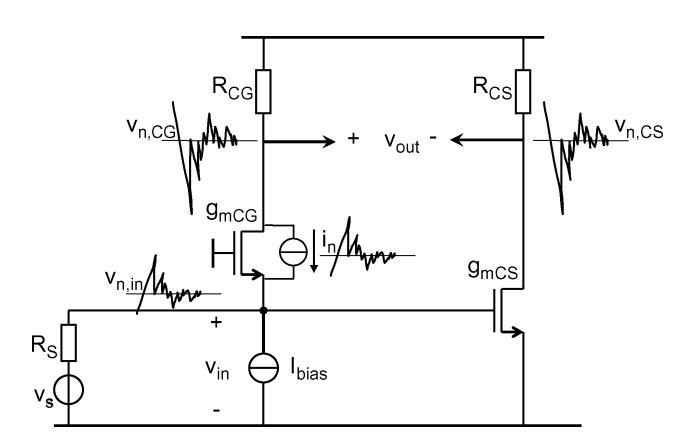
\includegraphics[width=\textwidth]{IMAGENS/blaakman_setup.png}
        \caption{Arquitetura ativa balun-LNA proposta.}
        \label{fig:LNA_noBuff}
    \end{subfigure}
    \hfill
    \begin{subfigure}[b]{0.45\textwidth}
        \centering
        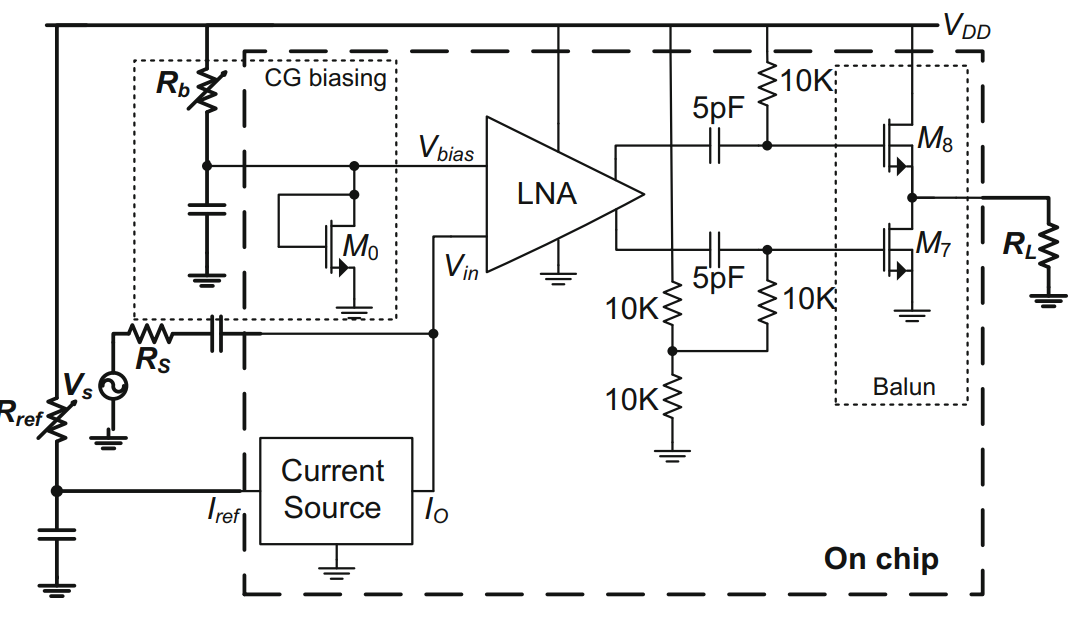
\includegraphics[width=\textwidth]{IMAGENS/balunBuffer.png}
        \caption{\textit{Buffer} de saída com cargas ativas.}
        \label{fig:bufferForLna}
    \end{subfigure}
    \caption{Circuito de referência estrutural para o desenvolvimento do LNA nas três tecnologias CMOS.}
    \label{fig:LNA_E_Buffer}
\end{figure}

O processo de dimensionamento partilha uma metodologia sistemática comum às três tecnologias abordadas. Contudo, a diferença 
fundamental reside nas dimensões características de cada nó tecnológico e na crescente relevância de efeitos de segundo ordem 
e canal curto, que deixam de ser desprezáveis à medida que as dimensões geométricas diminuem. No contexto de radiofrequência 
(RF), a adaptação de impedância às linhas de transmissão e interfaces de teste é sempre considerada uma restrição de projeto 
prioritária, sendo o objetivo garantir o casamento de impedâncias de entrada e saída ao valor padrão de $50~\Omega$.

\subsection*{Estágio \textit{common-gate}}

A impedância de entrada vista a partir do terminal de \textit{source} do transistor NMOS em configuração \textit{common-gate} 
é modelada analiticamente por

\begin{equation}
    Z_{\text{in}} = \frac{1}{g_m + g_{ds} + g_{mb}},
    \label{eq:zin}
\end{equation}

onde se inclui explicitamente o contributo da transcondutância de substrato (efeito de corpo) $g_{mb}$. Este parâmetro assume 
particular relevância nesta configuração uma vez que o terminal de \textit{bulk} se encontra tipicamente ligado ao potencial 
de referência (\textit{ground}), não acompanhando a excursão de sinal do terminal de \textit{source} ($V_{BS} \neq 0$). O fator 
dominante de projeto é a transcondutância de canal $g_m$, relacionada com a corrente de dreno em regime de saturação de canal 
longo por

\begin{equation}
    g_m = \frac{2 I_D}{V_{DS_{\text{sat}}}},
    \label{eq:gm}
\end{equation}

o que permite ajustar quantitativamente a impedância de entrada através da corrente de polarização DC, $I_{\text{bias}}$. Para 
que o casamento de impedância de entrada perfeito a $Z_{\text{in}} = 50~\Omega$ seja assegurado, é necessário que o denominador 
de~\eqref{eq:zin} convirja para a condutância alvo de $20~\text{mS}$. A tensão de \textit{bias} aplicada à \textit{gate} é fixada 
estaticamente a metade da tensão de alimentação nominal ($V_{DD}/2$) para maximizar a gama de excursão de sinal (*headroom*). O 
ganho de tensão em malha aberta deste estágio é expresso por

\begin{equation}
    A_{v_1} = \frac{g_m}{g_{ds} + g_{CG}}, \quad \text{onde } g_{CG} = \frac{1}{R_{CG}},
    \label{eq:av1}
\end{equation}

indicando que o valor da resistência de carga ativa ou passiva $R_{CG}$ constitui o principal parâmetro de ajuste e otimização 
do ganho de tensão. O procedimento de projeto consistiu em fixar um ganho-alvo equivalente ao Máximo Ganho Disponível (MAG) 
previamente obtido com a tecnologia bipolar BFP420, aproximando os resultados iterativamente com base na matriz de parâmetros S 
simulada.

\begin{figure}[H]
    \centering
    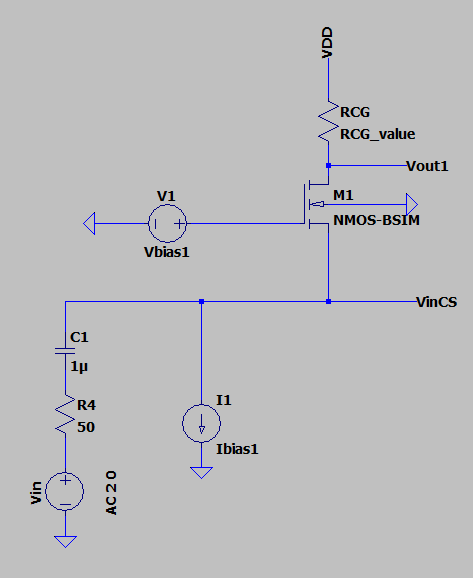
\includegraphics[width=0.42\textwidth]{IMAGENS/CommonGateSetup.png}
    \caption{Configuração \textit{common-gate} com realce da impedância de entrada intrínseca.}
    \label{fig:commonGate}
\end{figure}

\subsection*{Estágio \textit{common-source}}

O sinal de excitação de RF de entrada $V_{\text{in}}$ é partilhado em paralelo entre as duas configurações de transcondutância. 
A montagem \textit{common-source} introduz a inversão de fase necessária à funcionalidade de balun, apresentando um ganho de 
tensão de pequenos sinais dado por

\begin{equation}
    A_{v_2} = -\frac{g_m}{g_{ds} + g_{CS}}, \quad \text{onde } g_{CS} = \frac{1}{R_{CS}}.
    \label{eq:av2}
\end{equation}

Para isolar os pontos de operação DC de polarização de cada estágio independente, é inserido um condensador de acoplamento de 
valor elevado entre as duas montagens, mitigando interferências mútuas na rede de polarização. O equilíbrio de ganho diferencial 
e o ajuste do ponto de operação neste estágio são realizados através da variação fina da tensão de \textit{gate}, controlando a 
tensão de \textit{overdrive} $V_{OV} = V_{GS} - V_{th}$ e, por conseguinte, a densidade de corrente de dreno do dispositivo.

\begin{figure}[H]
    \centering
    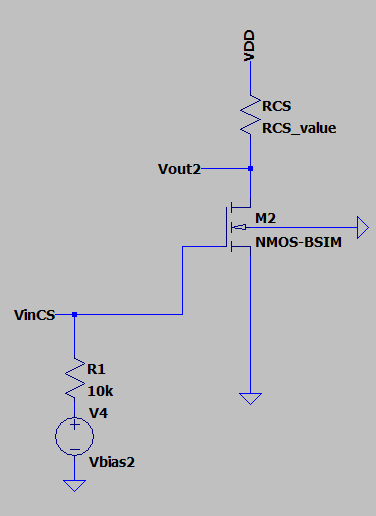
\includegraphics[width=0.42\textwidth]{IMAGENS/CommonSourceSetup.png}
    \caption{Configuração \textit{common-source} responsável pela inversão de fase na conversão diferencial.}
    \label{fig:commonSource}
\end{figure}

O fator de escala geométrico $n$, aplicado de forma simétrica às dimensões de largura ($W$) dos transistores centrais do LNA, 
permite estabelecer um compromisso ótimo (\textit{trade-off}) entre o ganho de transcondutância, as capacidades parasitas 
intrínsecas e a figura de ruído. No âmbito deste projeto, o fator de escala nominal foi fixado em $n = 2{,}75$, tendo-se 
posteriormente estendido a análise paramétrica aos valores de $n \in \{1;\ 2;\ 2{,}75;\ 3{,}5\}$ de modo a mapear a sensibilidade 
do desempenho global face à variação da área ativa dos dispositivos.

\subsection*{Estágio de saída com \textit{buffer} de cargas ativas}

A impedância de saída de pequenos sinais do estágio de \textit{buffer} resulta do paralelo entre a impedância vista pelo dreno 
do transistor inferior (fonte de corrente ativa) e a impedância de saída vista pela \textit{source} do transistor superior 
(configuração seguidor de fonte ou \textit{source follower}):

\begin{equation}
    Z_{\text{out}} = \frac{1}{g_{m_{\text{up}}} + g_{ds_{\text{up}}} + g_{ds_{\text{dn}}}}.
    \label{eq:zout}
\end{equation}

Esta configuração providencia um isolamento reverso elevado, minimizando os efeitos de carga do estágio de mistura posterior 
sobre o núcleo amplificador do LNA, garantindo simultaneamente o casamento de saída para os $50~\Omega$ instrumentais através 
do ajuste geométrico da transcondutância $g_{m_{\text{up}}}$.

\begin{figure}[H]
    \centering
    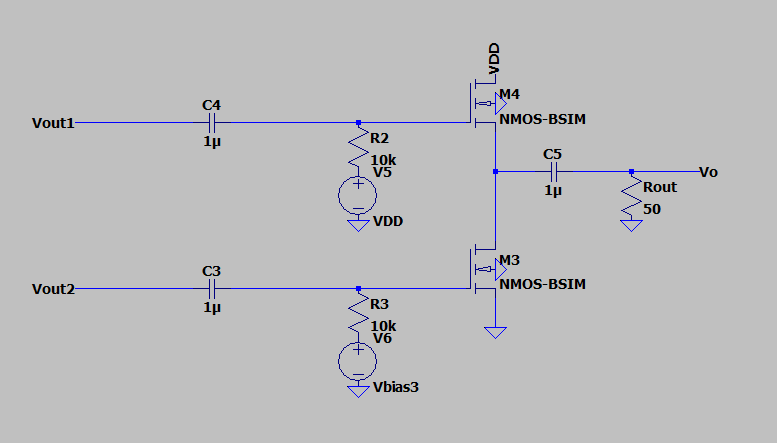
\includegraphics[width=0.42\textwidth]{IMAGENS/BufferSetup.png}
    \caption{\textit{Buffer} diferencial de cargas ativas e respetiva topologia de impedância de saída.}
    \label{fig:bufferSetup}
\end{figure}

% ============================================================
\subsection{CMOS de 350\,nm}
% ============================================================

Na tecnologia de 350\,nm, o comprimento físico do canal apresenta dimensões superiores à escala de sub-mícron profundo, 
permitindo classificar o dispositivo analógico como pertencente ao regime de canal longo. Consequentemente, as equações clássicas 
de primeira ordem baseadas no modelo quadrático mantêm um elevado grau de previsibilidade e validade para o dimensionamento em RF.
 Os efeitos secundários de canal curto, tais como a saturação de velocidade e a modulação do comprimento de canal por DIBL (\textit{Drain-Induced Barrier Lowering}), exercem uma influência reduzida nas figuras de mérito do transístor.

\begin{figure}[H]
    \centering
    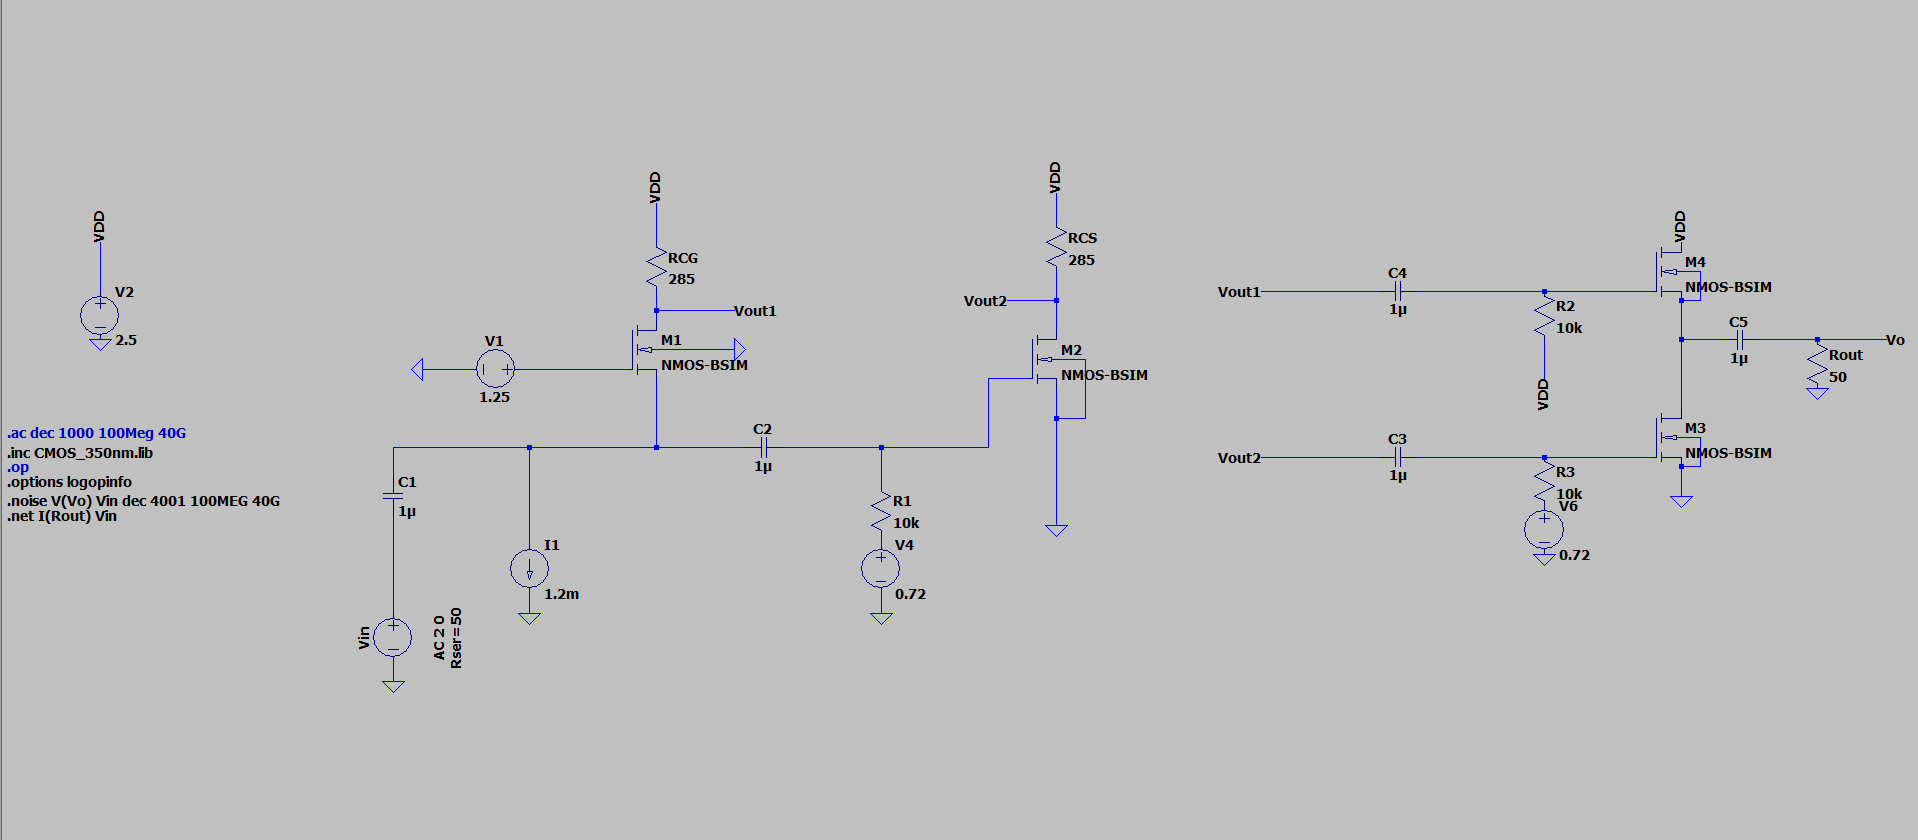
\includegraphics[width=0.45\textwidth]{IMAGENS/ltspice350nm/CMOS350nm_schematic.png}
    \caption{Esquemático elétrico do LNA completo implementado na plataforma LTspice utilizando tecnologia CMOS de 350\,nm.}
    \label{fig:350nmLNA}
\end{figure}

Os resultados relativos à resposta de ruído e aos pontos de operação DC do circuito polarizado são analisados de seguida para 
cada fator de escala $n$. Nesta tecnologia, o desempenho espetral de ruído e as curvas de ganho foram extraídos via simulação AC 
e as grandezas operacionais DC foram obtidas diretamente a partir do relatório \texttt{.op} gerado pelo motor SPICE. 

Os resultados da simulação dos parâmetros S indicam que os coeficientes de reflexão à entrada ($S_{11}$) e à saída ($S_{22}$) se 
situam consistentemente abaixo do limiar crítico de $-10\text{ dB}$ na banda de interesse, validando a metodologia de casamento 
de impedâncias. Adicionalmente, verifica-se uma alteração incremental no perfil de desempenho à medida que o fator de escala é 
majorado. Este comportamento decorre do facto de a variação geométrica da largura ($W$) redefinir as capacidades intrínsecas de 
porta ($C_{gs}$, $C_{gd}$) e as condutâncias de saída ($g_{ds}$), deslocando ligeiramente o ponto ótimo de ruído e de adaptação 
relativamente ao centro da banda projetada.

\subsubsection{Fator de escala \texorpdfstring{$N = 1$}{N=1}}

\begin{figure}[H]
    \centering
    \begin{subfigure}[b]{0.48\textwidth}
        \centering
        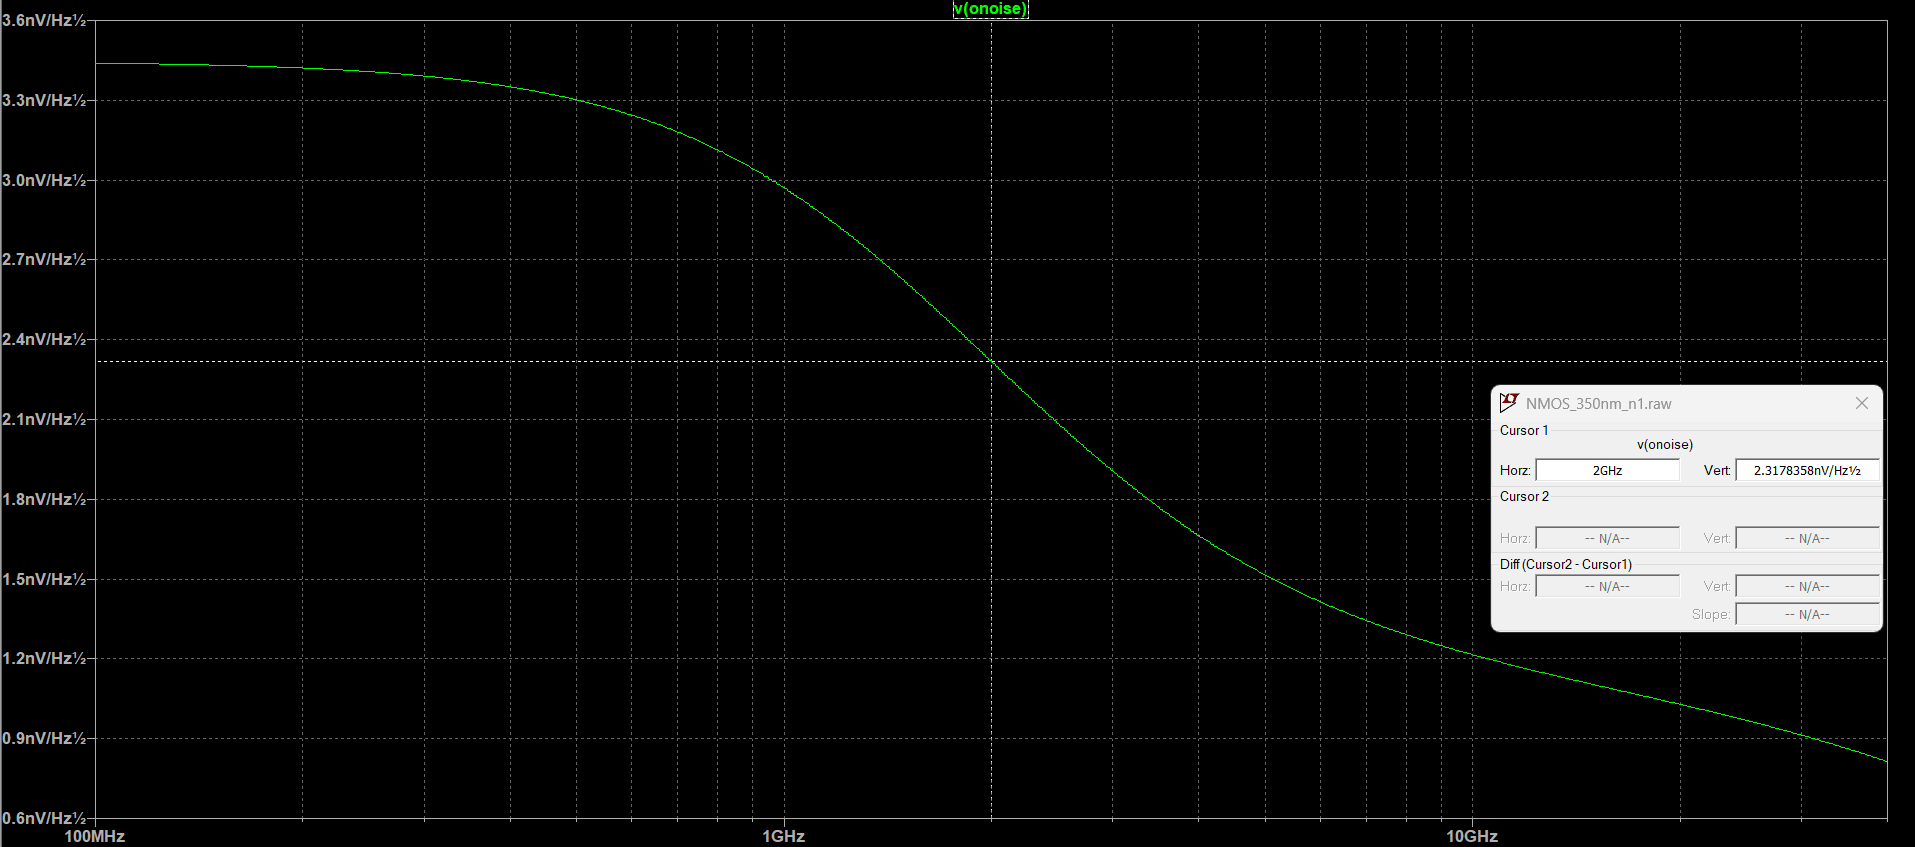
\includegraphics[width=\textwidth]{IMAGENS/ltspice350nm/CMOS350nm_N1_noise.png}
        \caption{Espetro de densidade de ruído.}
        \label{fig:noise350_N1}
    \end{subfigure}
    \hfill
    \begin{subfigure}[b]{0.48\textwidth}
        \centering
        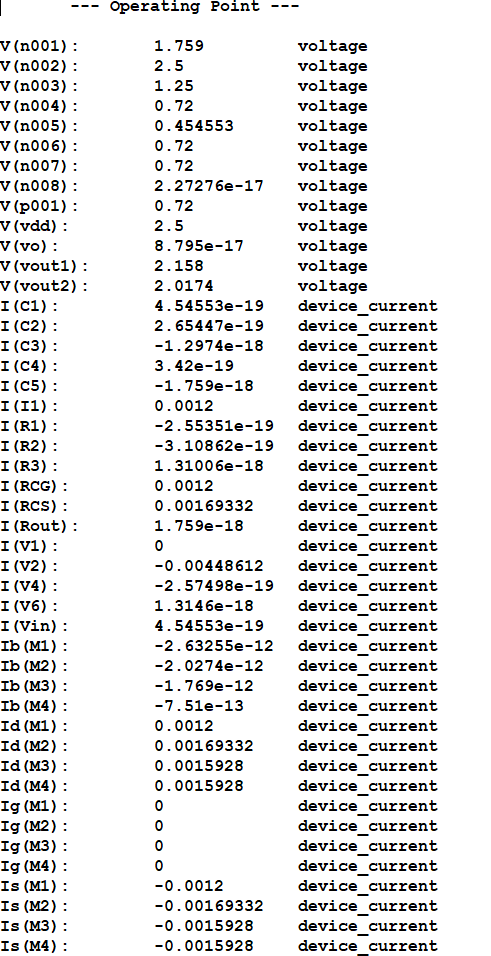
\includegraphics[width=\textwidth]{IMAGENS/ltspice350nm/CMOS350nm_N1_DCop.png}
        \caption{Ponto de operação DC do simulador.}
        \label{fig:op350_N1}
    \end{subfigure}
    \vskip\baselineskip
    \begin{subfigure}[c]{0.48\textwidth}
        \centering
        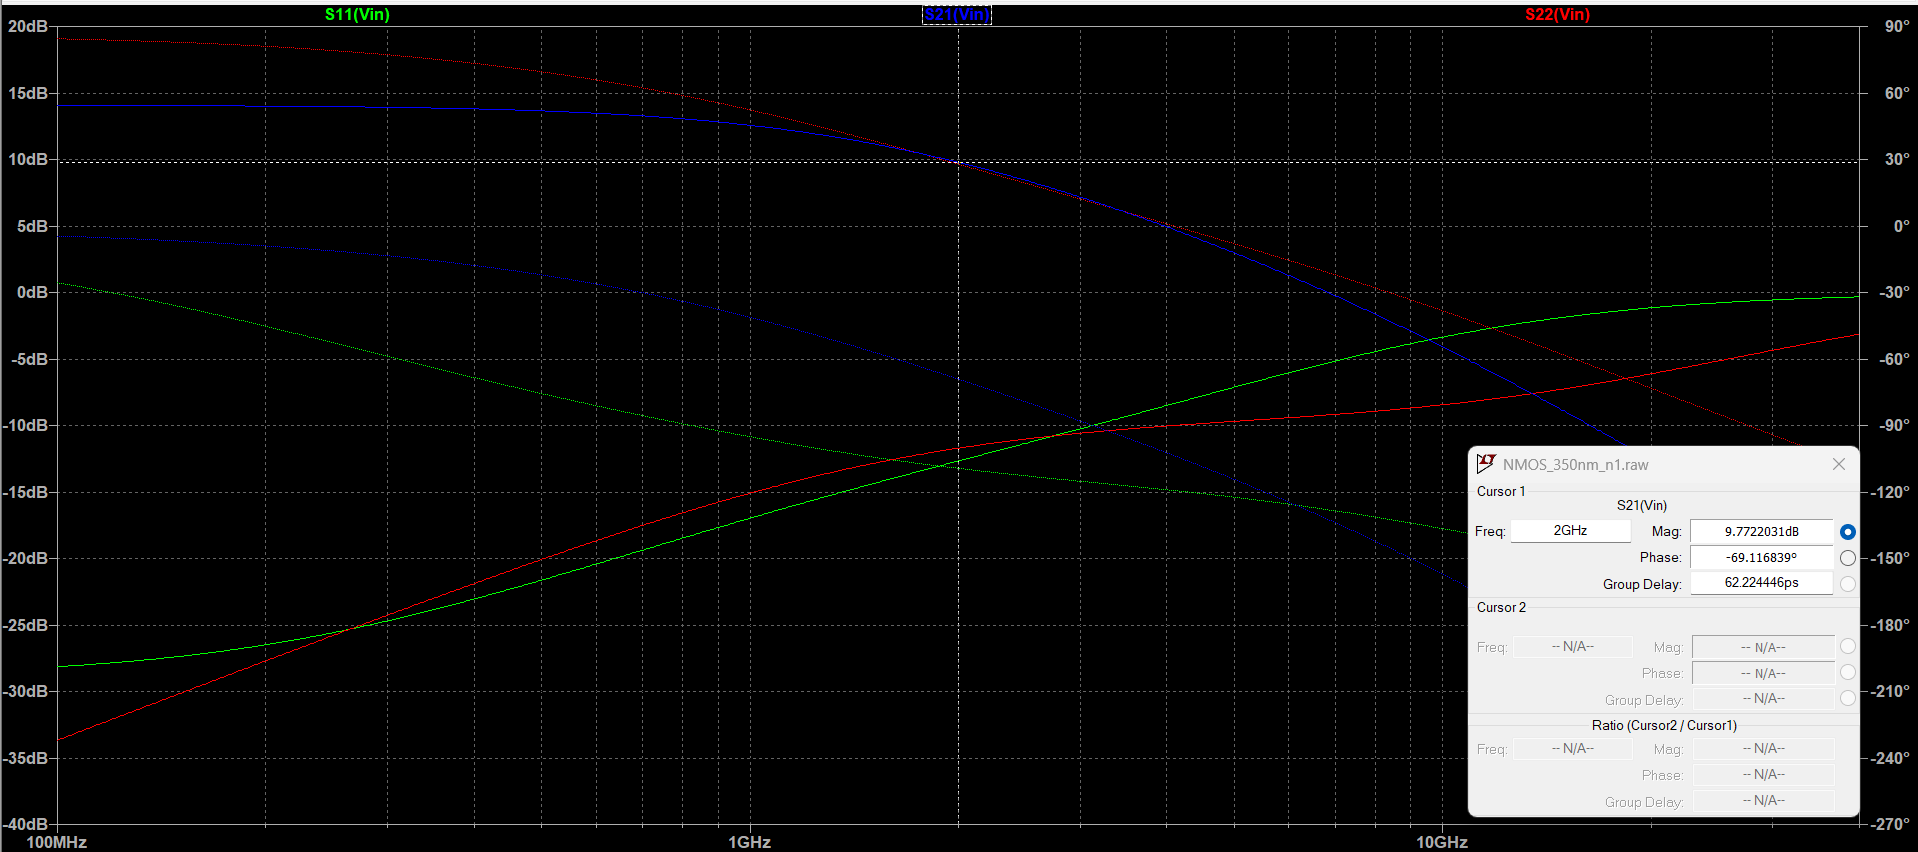
\includegraphics[width=\textwidth]{IMAGENS/ltspice350nm/CMOS350nm_N1_gainSparam.png}
        \caption{Resposta em frequência dos parâmetros S.}
        \label{fig:gain350_N1}
    \end{subfigure}
    \caption{Análise espetral de ruído, ponto de operação DC e coeficientes de transmissão/reflexão para $N=1$ em tecnologia CMOS 
    de 350\,nm na gama de 100\,MHz a 2\,GHz.}
\end{figure}

\subsubsection{Fator de escala \texorpdfstring{$N = 2$}{N=2}}

\begin{figure}[H]
    \centering
    \begin{subfigure}[b]{0.48\textwidth}
        \centering
        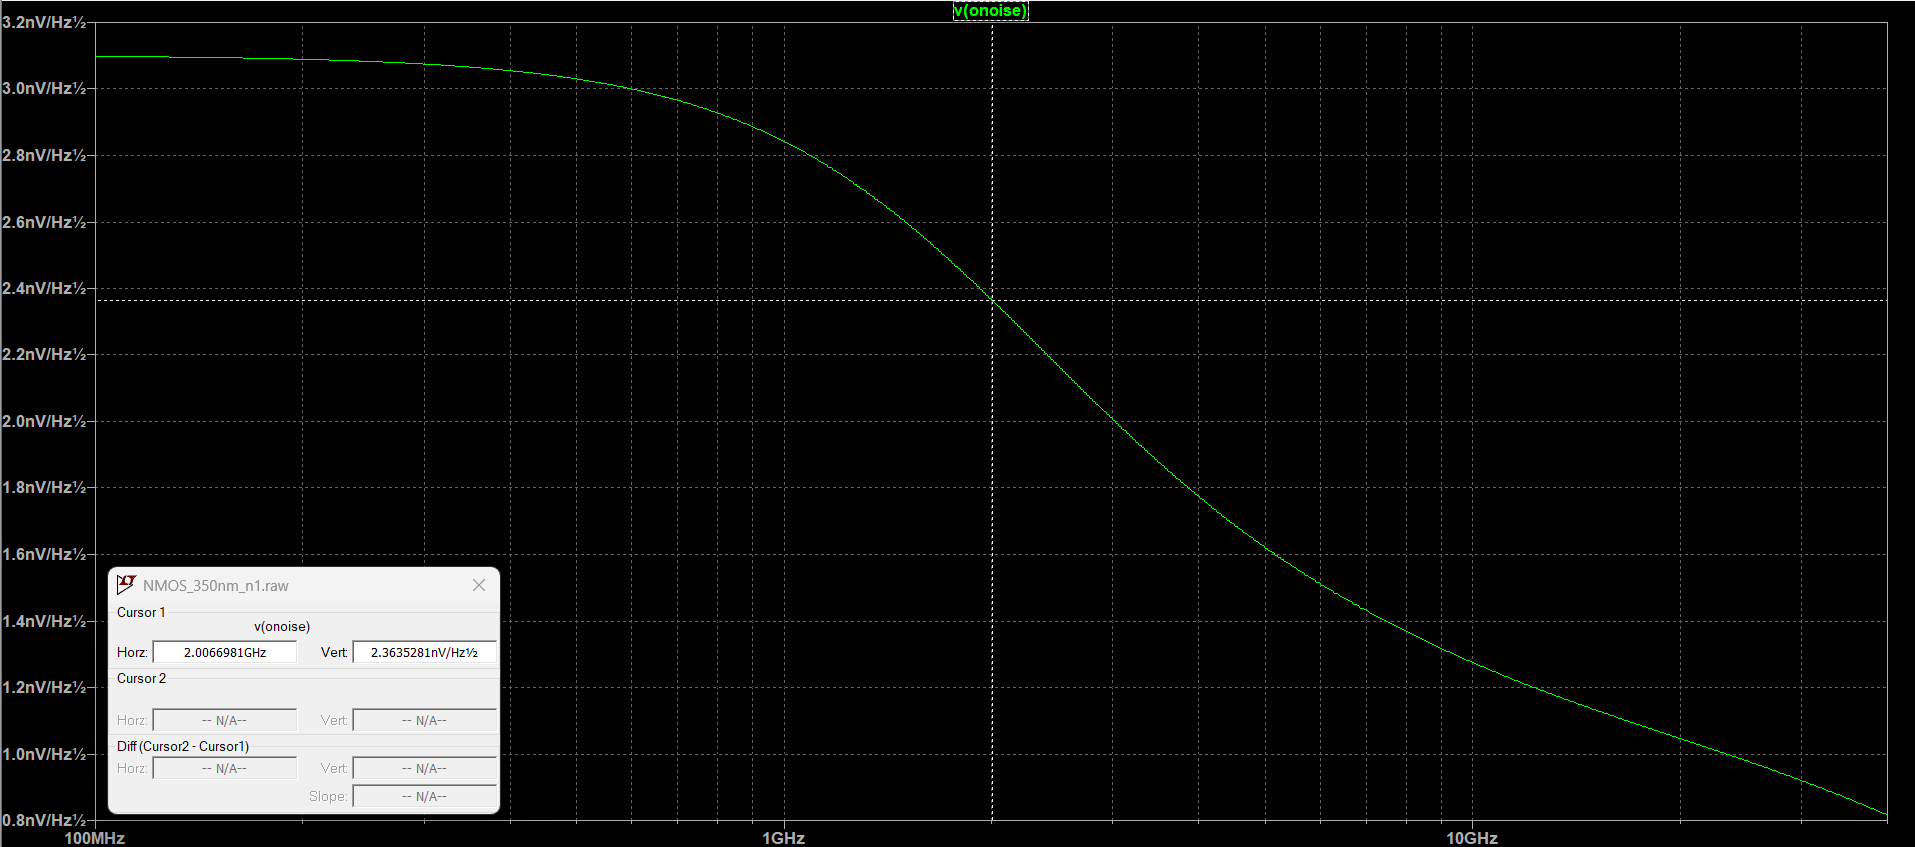
\includegraphics[width=\textwidth]{IMAGENS/ltspice350nm/CMOS350nm_N2_noise.png}
        \caption{Espetro de densidade de ruído.}
        \label{fig:noise350_N2}
    \end{subfigure}
    \hfill
    \begin{subfigure}[b]{0.48\textwidth}
        \centering
        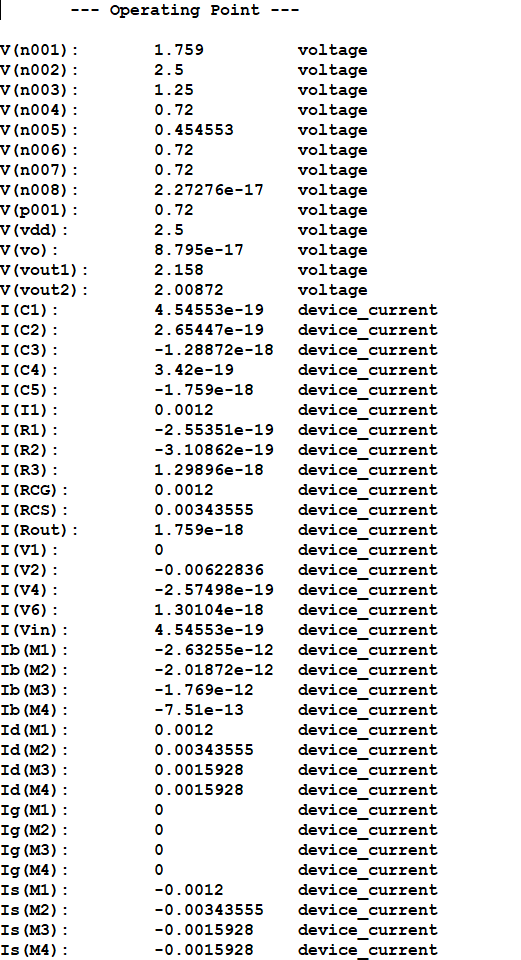
\includegraphics[width=\textwidth]{IMAGENS/ltspice350nm/CMOS350nm_N2_DCop.png}
        \caption{Ponto de operação DC do simulador.}
        \label{fig:op350_N2}
    \end{subfigure}
    \vskip\baselineskip
    \begin{subfigure}[c]{0.48\textwidth}
        \centering
        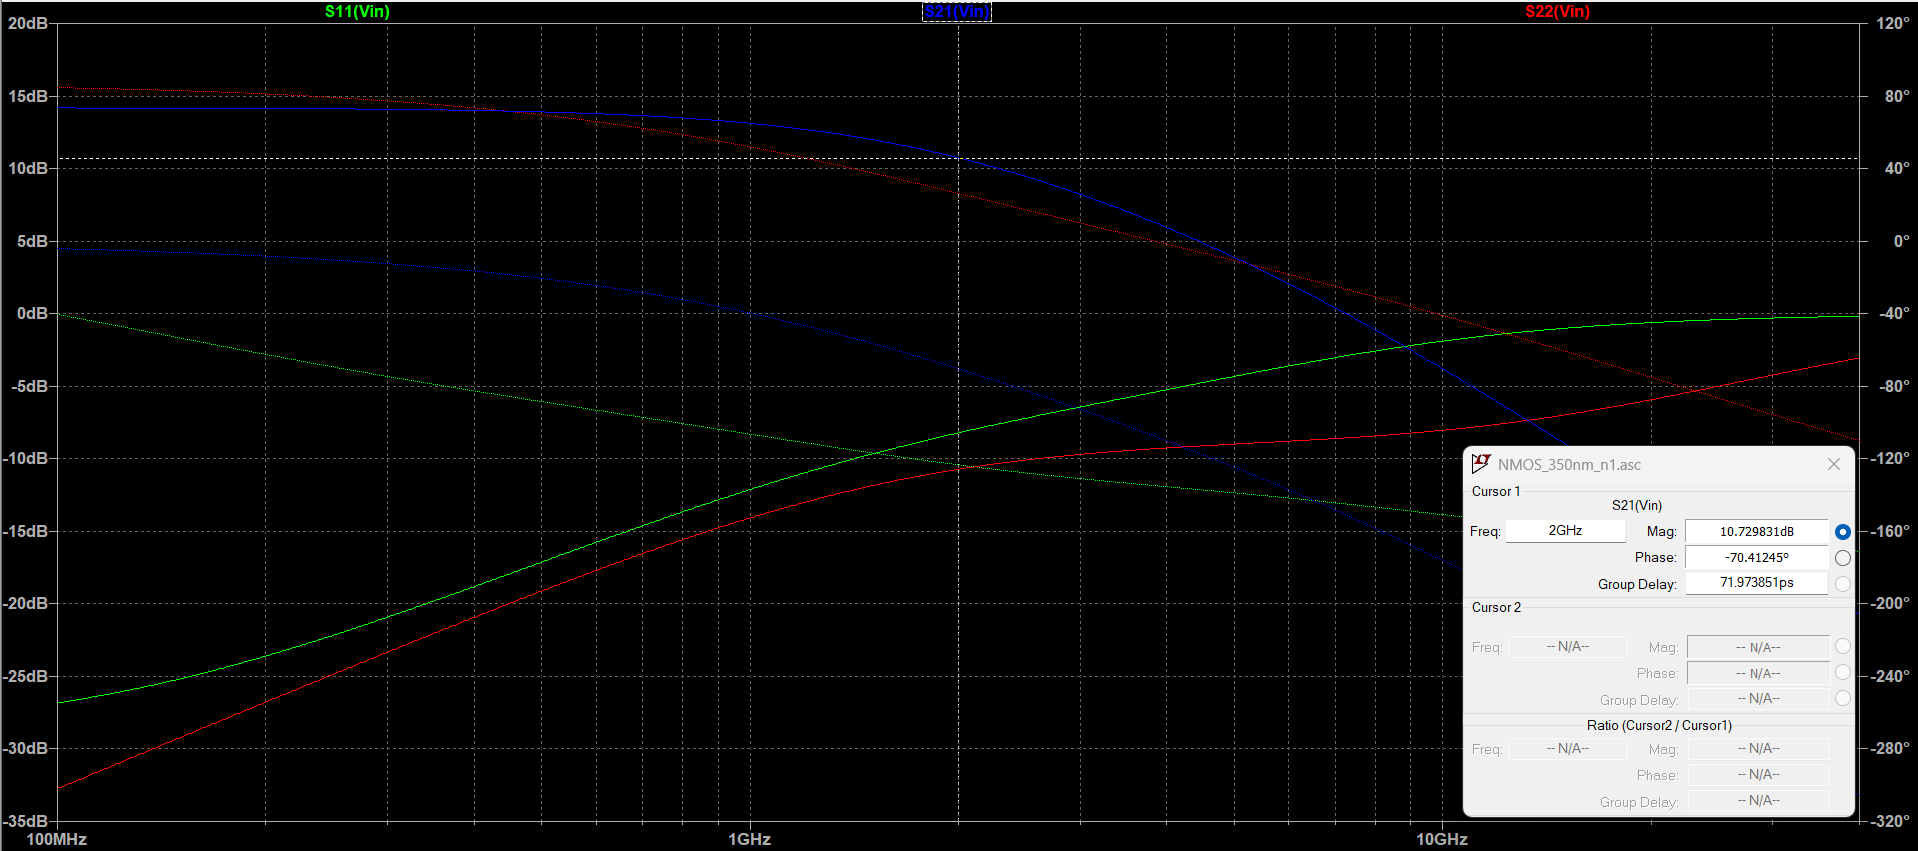
\includegraphics[width=\textwidth]{IMAGENS/ltspice350nm/CMOS350nm_N2_gainSparam.png}
        \caption{Resposta em frequência dos parâmetros S.}
        \label{fig:gain350_N2}
    \end{subfigure}
    \caption{Análise espetral de ruído, ponto de operação DC e coeficientes de transmissão/reflexão para $N=2$ em tecnologia CMOS 
    de 350\,nm na gama de 100\,MHz a 2\,GHz.}
\end{figure}

\subsubsection{Fator de escala \texorpdfstring{$N = 2{,}75$}{N=2.75}}

\begin{figure}[H]
    \centering
    \begin{subfigure}[b]{0.48\textwidth}
        \centering
        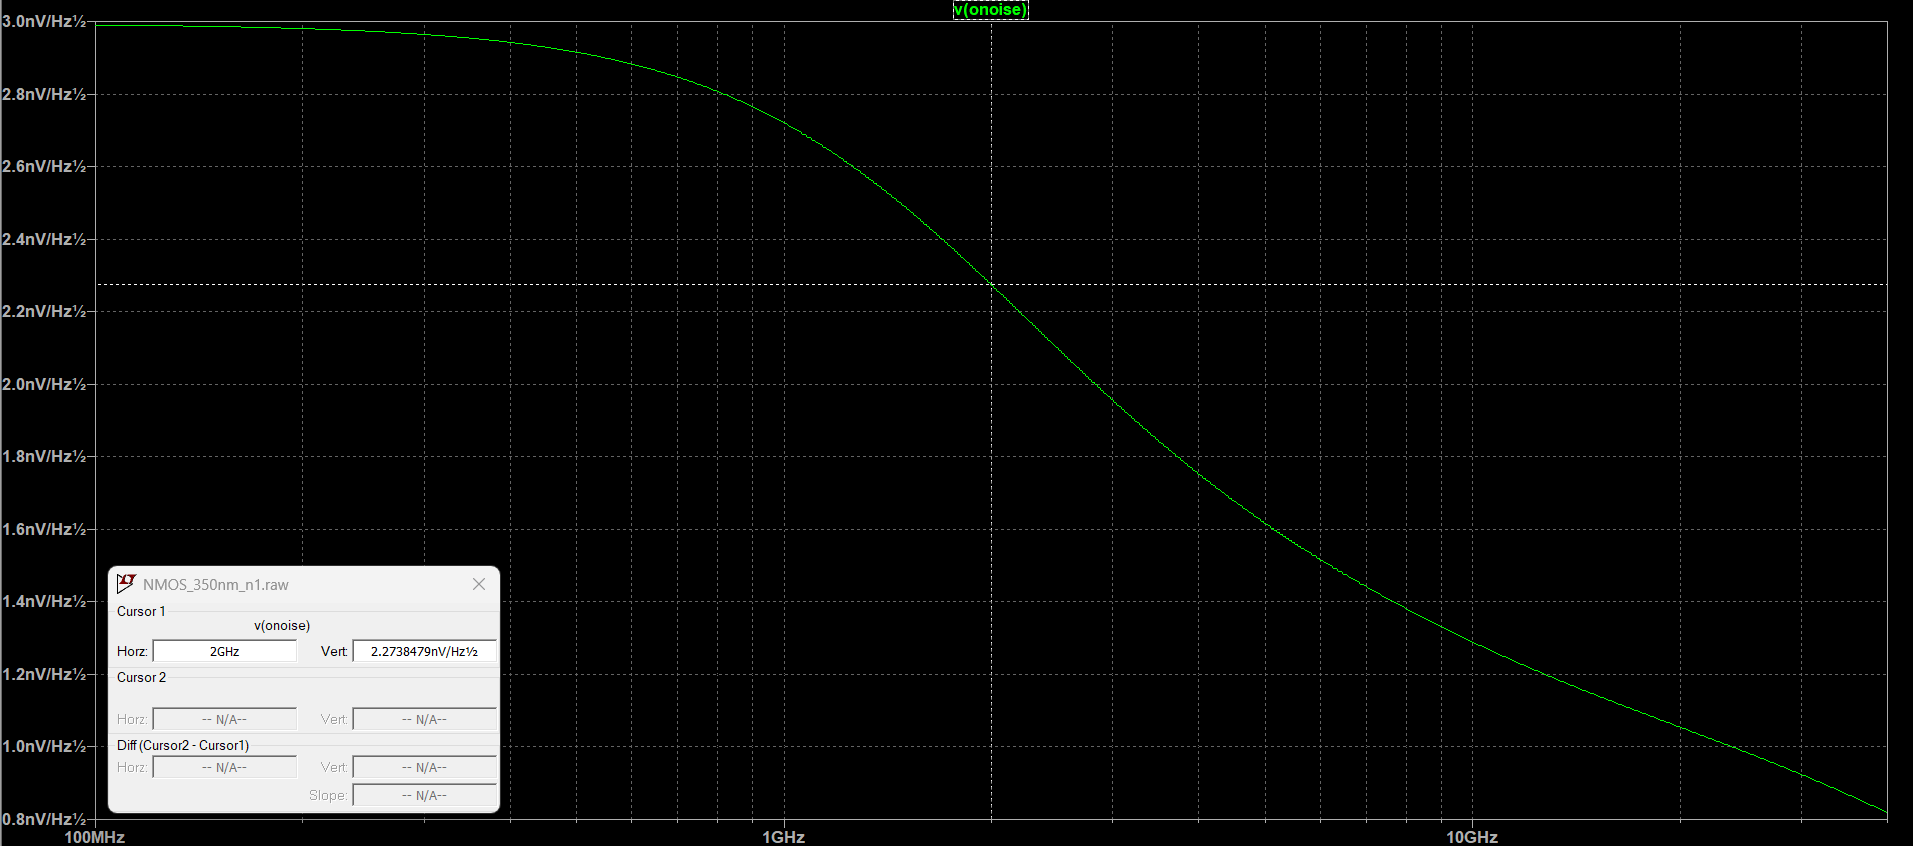
\includegraphics[width=\textwidth]{IMAGENS/ltspice350nm/CMOS350nm_N275_noise.png}
        \caption{Espetro de densidade de ruído.}
        \label{fig:noise350_N275}
    \end{subfigure}
    \hfill
    \begin{subfigure}[b]{0.48\textwidth}
        \centering
        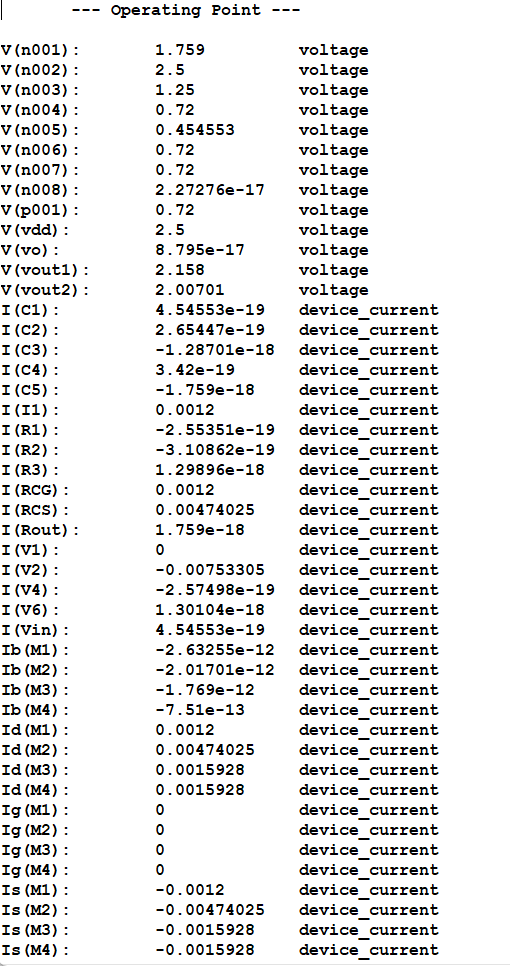
\includegraphics[width=\textwidth]{IMAGENS/ltspice350nm/CMOS350nm_N275_DCop.png}
        \caption{Ponto de operação DC do simulador.}
        \label{fig:op350_N275}
    \end{subfigure}
    \vskip\baselineskip
    \begin{subfigure}[c]{0.48\textwidth}
        \centering
        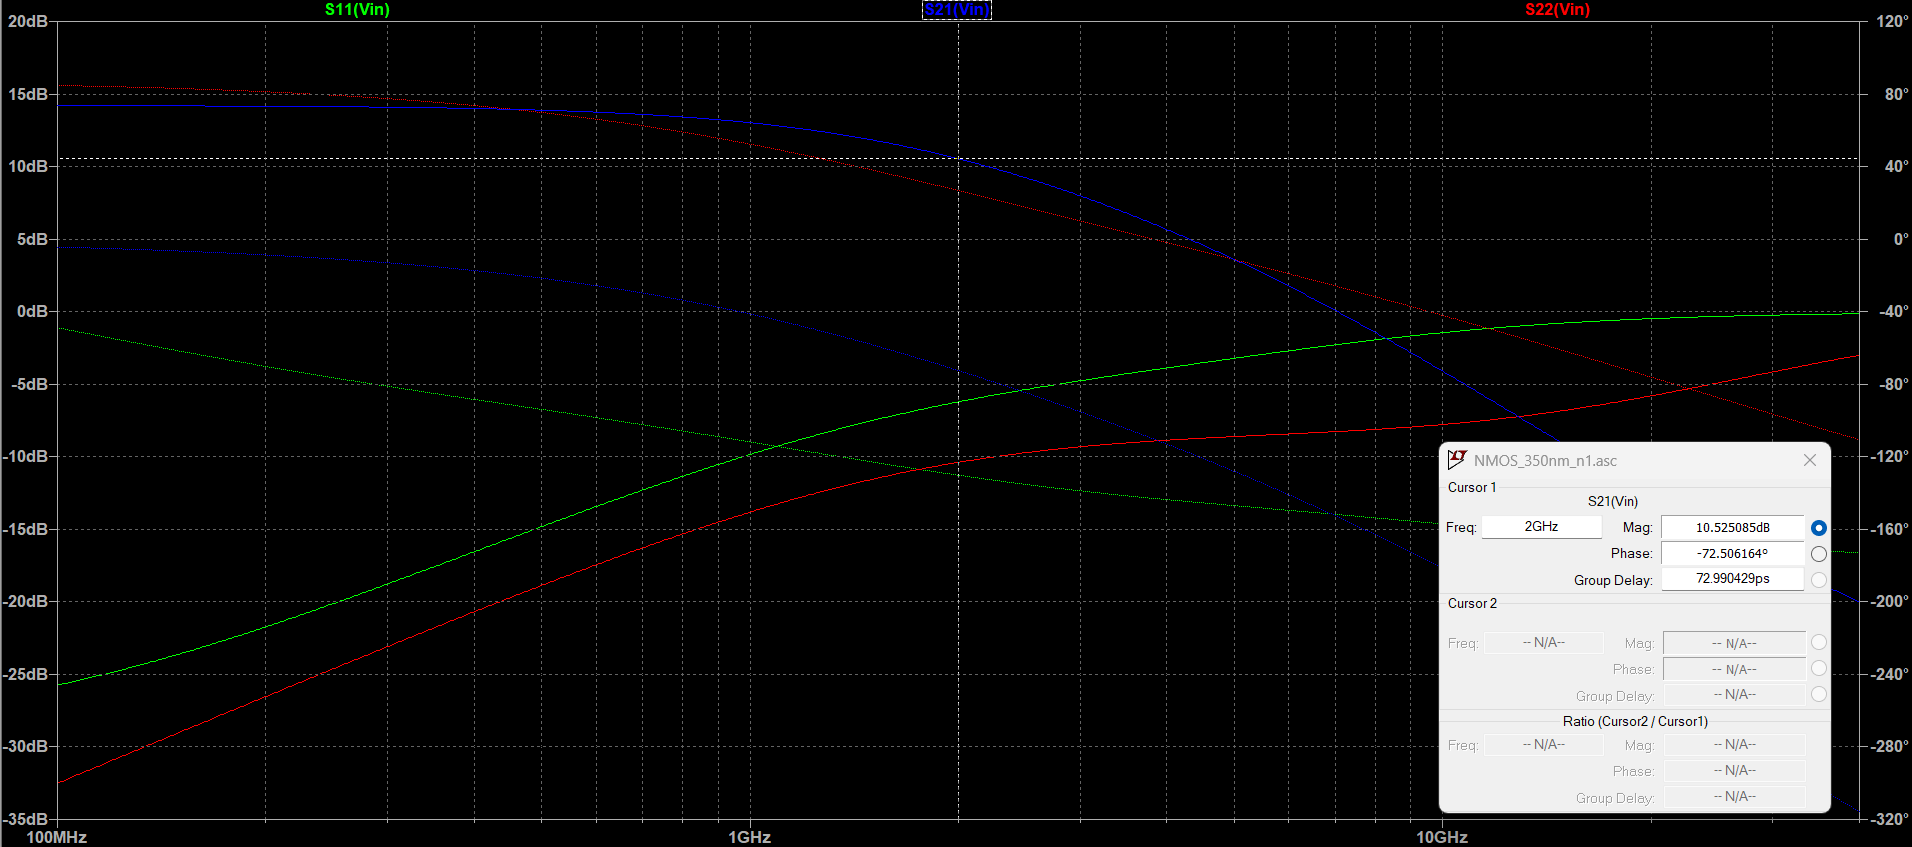
\includegraphics[width=\textwidth]{IMAGENS/ltspice350nm/CMOS350nm_N275_gainSparam.png}
        \caption{Resposta em frequência dos parâmetros S.}
        \label{fig:gain350_N275}
    \end{subfigure}
    \caption{Análise espetral de ruído, ponto de operação DC e coeficientes de transmissão/reflexão para o fator de escala de 
    grupo $N=2{,}75$ em tecnologia CMOS de 350\,nm na gama de 100\,MHz a 2\,GHz.}
\end{figure}

\subsubsection{Fator de escala \texorpdfstring{$N = 3{,}5$}{N=3.5}}

\begin{figure}[H]
    \centering
    \begin{subfigure}[b]{0.48\textwidth}
        \centering
        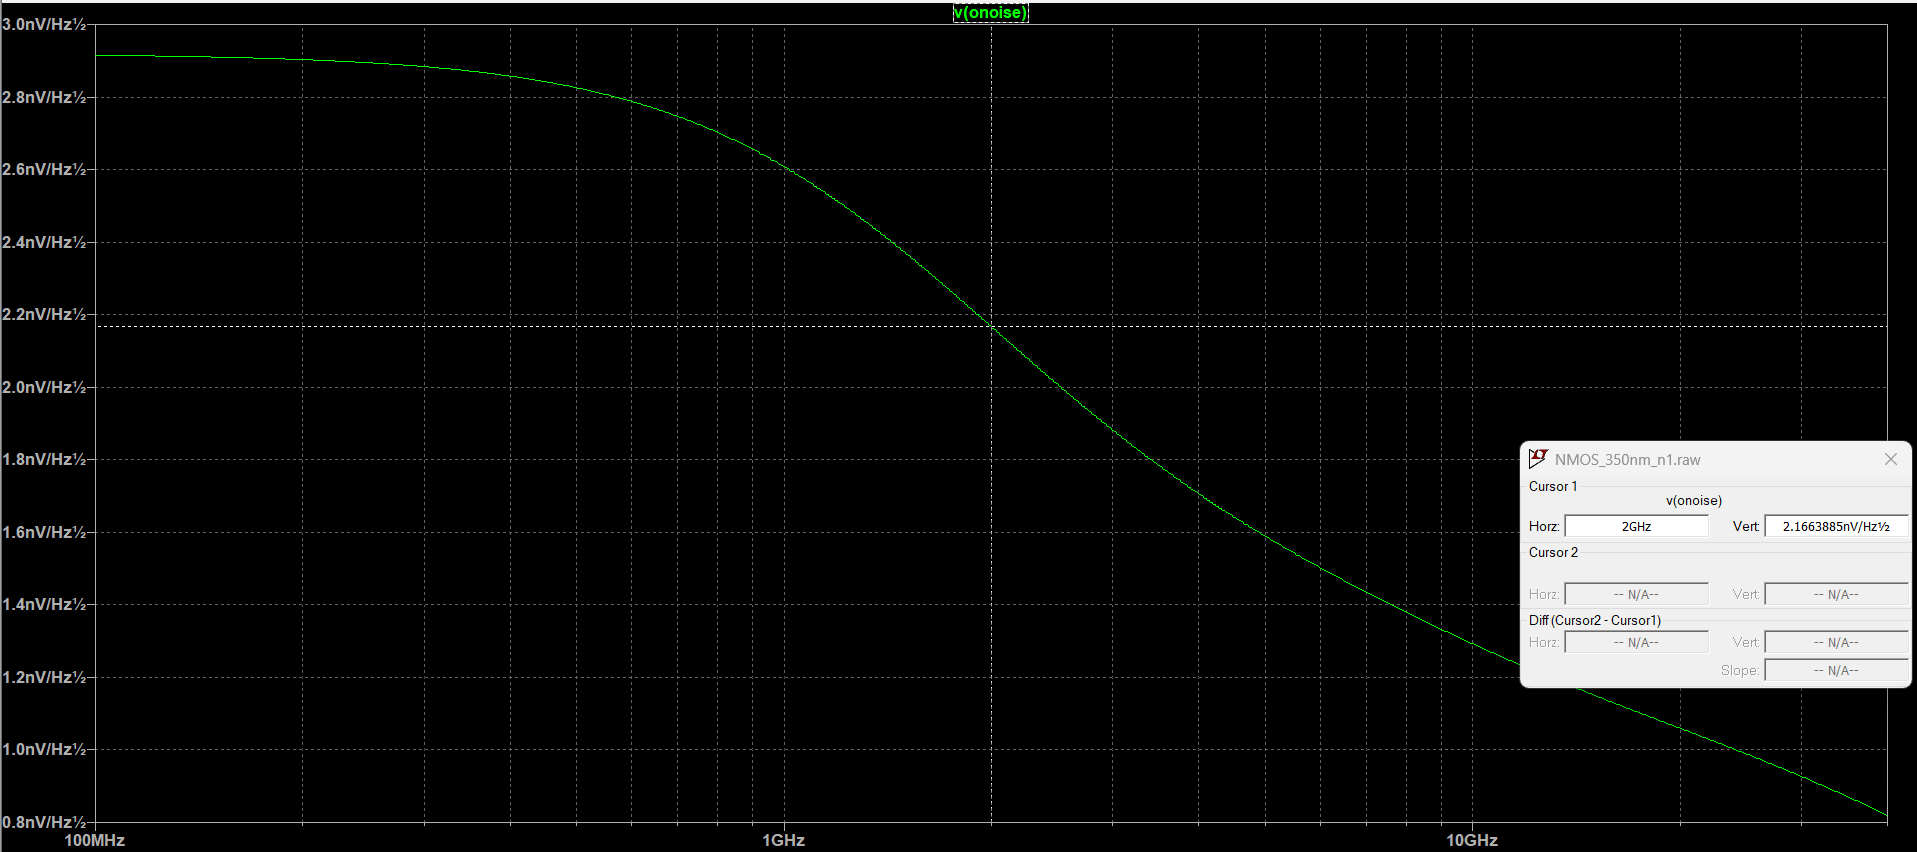
\includegraphics[width=\textwidth]{IMAGENS/ltspice350nm/CMOS350nm_N35_noise.png}
        \caption{Espetro de densidade de ruído.}
        \label{fig:noise350_N35}
    \end{subfigure}
    \hfill
    \begin{subfigure}[b]{0.48\textwidth}
        \centering
        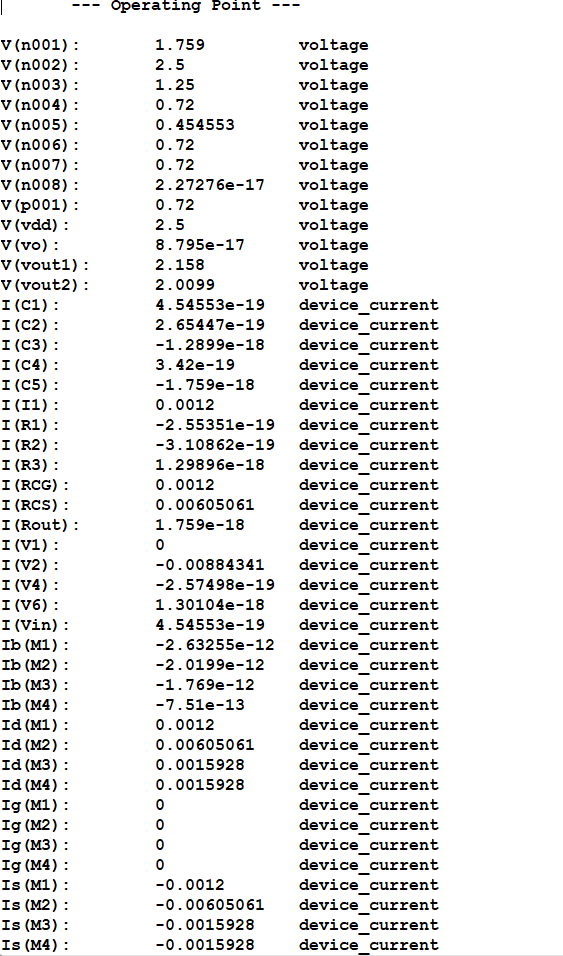
\includegraphics[width=\textwidth]{IMAGENS/ltspice350nm/CMOS350nm_N35_DCop.png}
        \caption{Ponto de operação DC do simulador.}
        \label{fig:op350_N35}
    \end{subfigure}
    \vskip\baselineskip
    \begin{subfigure}[c]{0.48\textwidth}
        \centering
        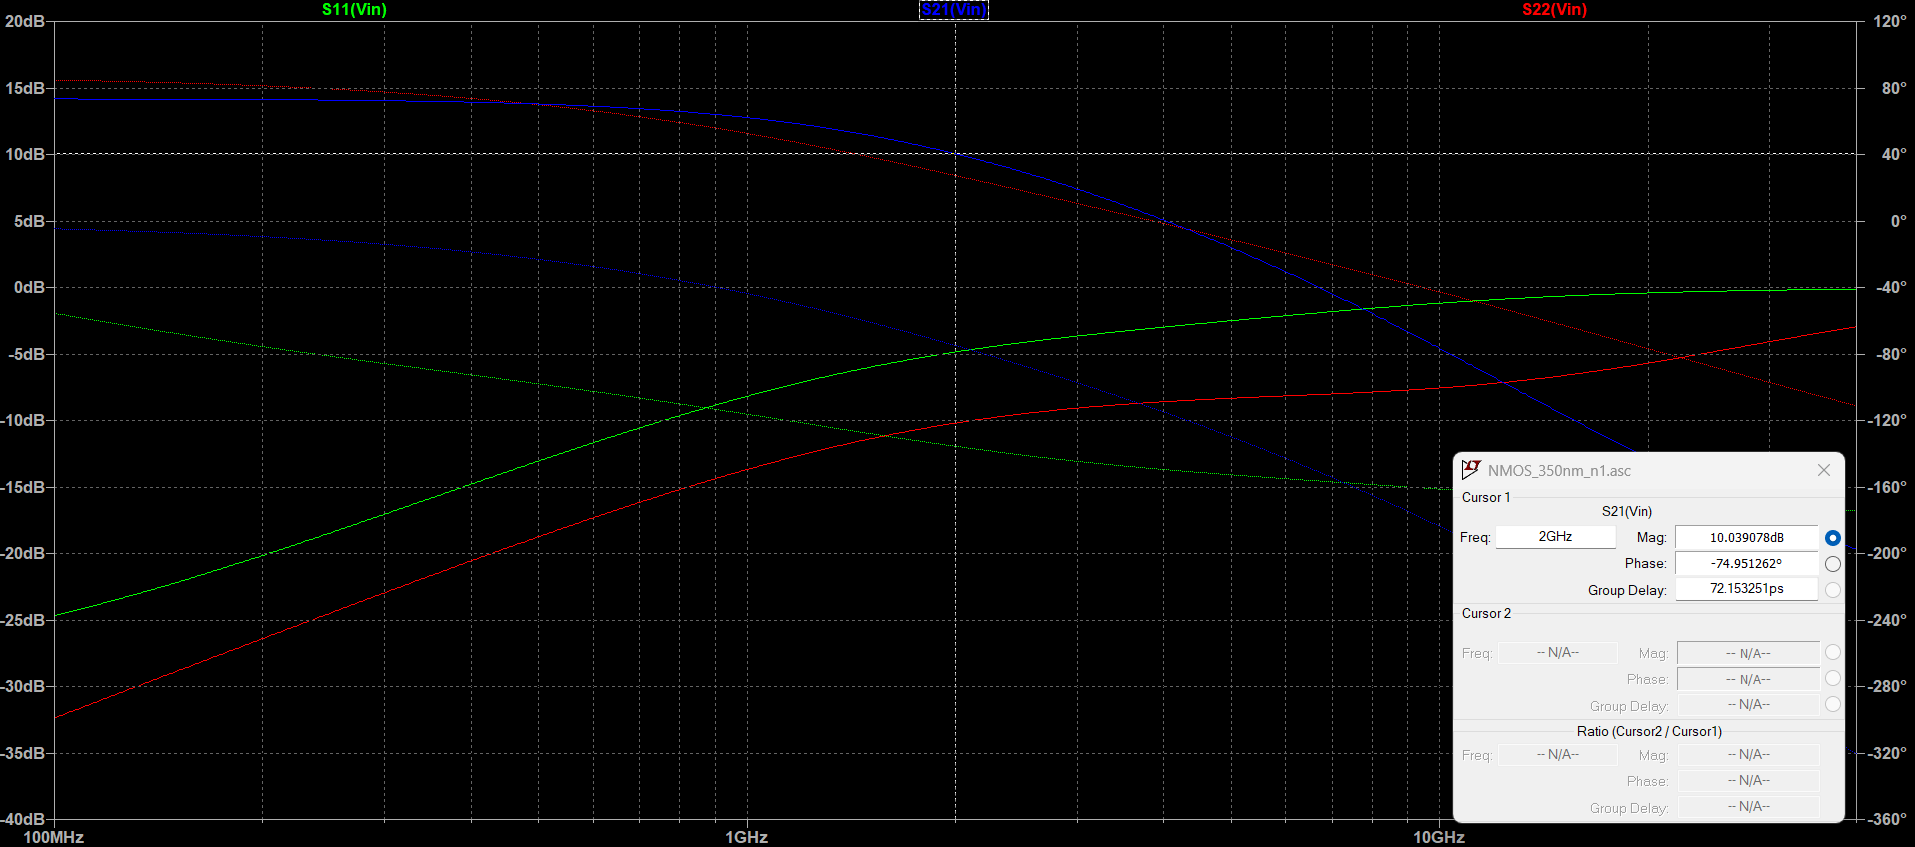
\includegraphics[width=\textwidth]{IMAGENS/ltspice350nm/CMOS350nm_N35_gainSparam.png}
        \caption{Resposta em frequência dos parâmetros S.}
        \label{fig:gain350_N35}
    \end{subfigure}
    \caption{Análise espetral de ruído, ponto de operação DC e coeficientes de transmissão/reflexão para $N=3{,}5$ em tecnologia 
    CMOS de 350\,nm na gama de 100\,MHz a 2\,GHz.}
\end{figure}

% ============================================================
\subsection{CMOS de 65\,nm}
% ============================================================

A tecnologia de 65\,nm representa o limiar crítico de transição entre o regime clássico de canal longo e o domínio de canal curto 
profundo (*deep sub-micron*). Sob estas condições, o dimensionamento analítico baseado em equações de primeira ordem atua 
meramente como uma aproximação elementar, uma vez que fenómenos físicos severos como a saturação de velocidade dos portadores de 
carga, a degradação da mobilidade efetiva devido ao campo elétrico vertical intenso e o aumento resistivo da \textit{gate} 
distribuída ($r_g$) passam a dominar as figuras de mérito de ruído e ganho. Por conseguinte, torna-se imperativo recorrer a uma 
caracterização rigorosa das propriedades físicas DC e da repartição detalhada das fontes de ruído intrínsecas a este nó 
tecnológico.

\begin{figure}[H]
    \centering
    \begin{subfigure}[b]{0.45\textwidth}
        \centering
        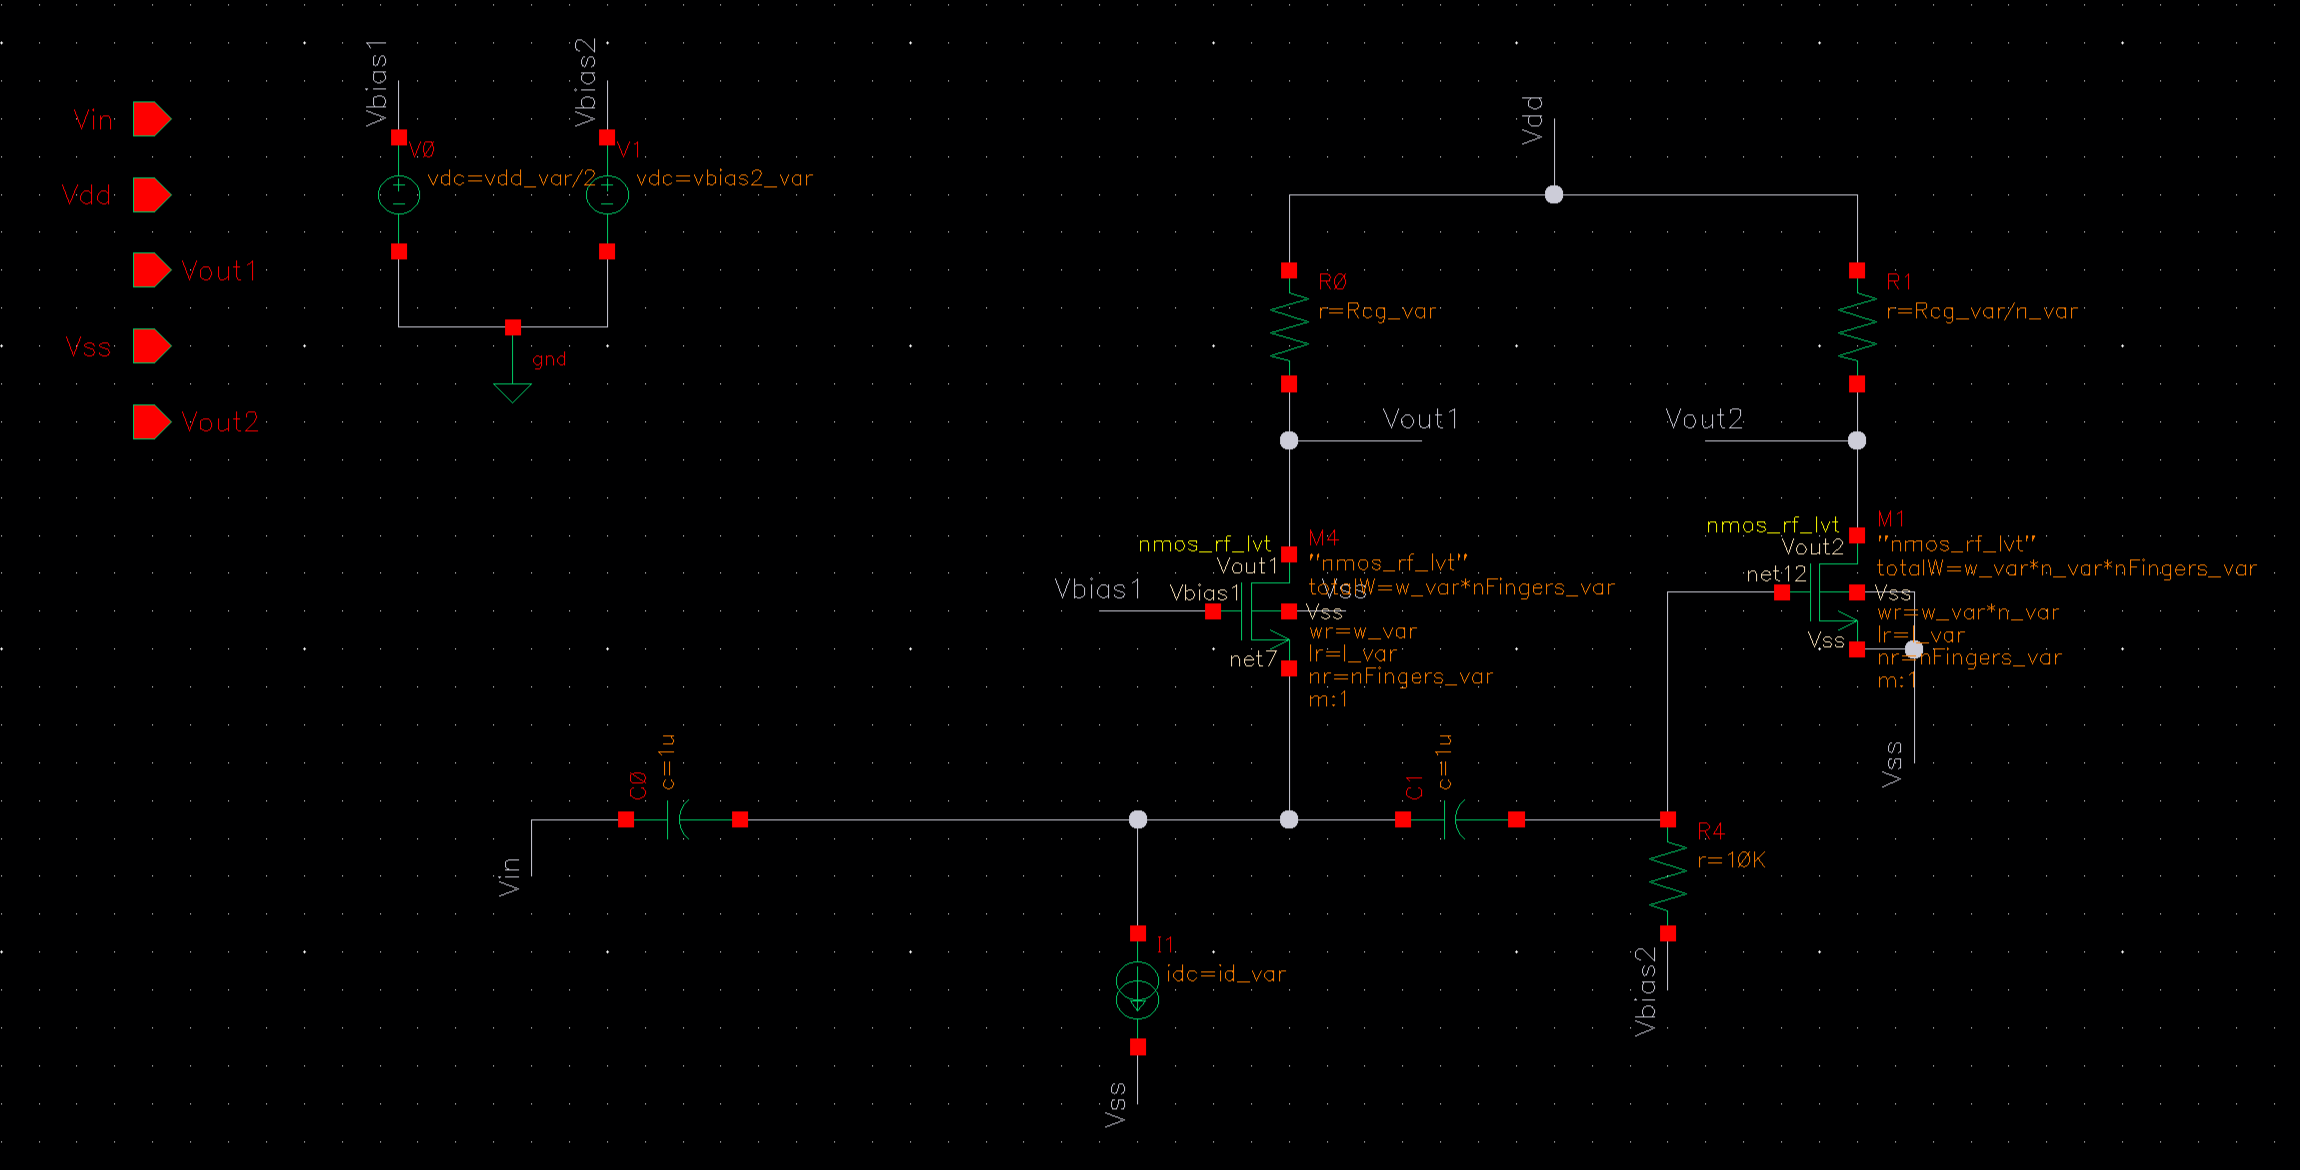
\includegraphics[width=\textwidth]{IMAGENS/cadence65nm/CMOS65_LNA_Lab1_Schematic.png}
        \caption{Estágio de transcondutância core do LNA.}
        \label{fig:LNA_65nm}
    \end{subfigure}
    \hfill
    \begin{subfigure}[b]{0.45\textwidth}
        \centering
        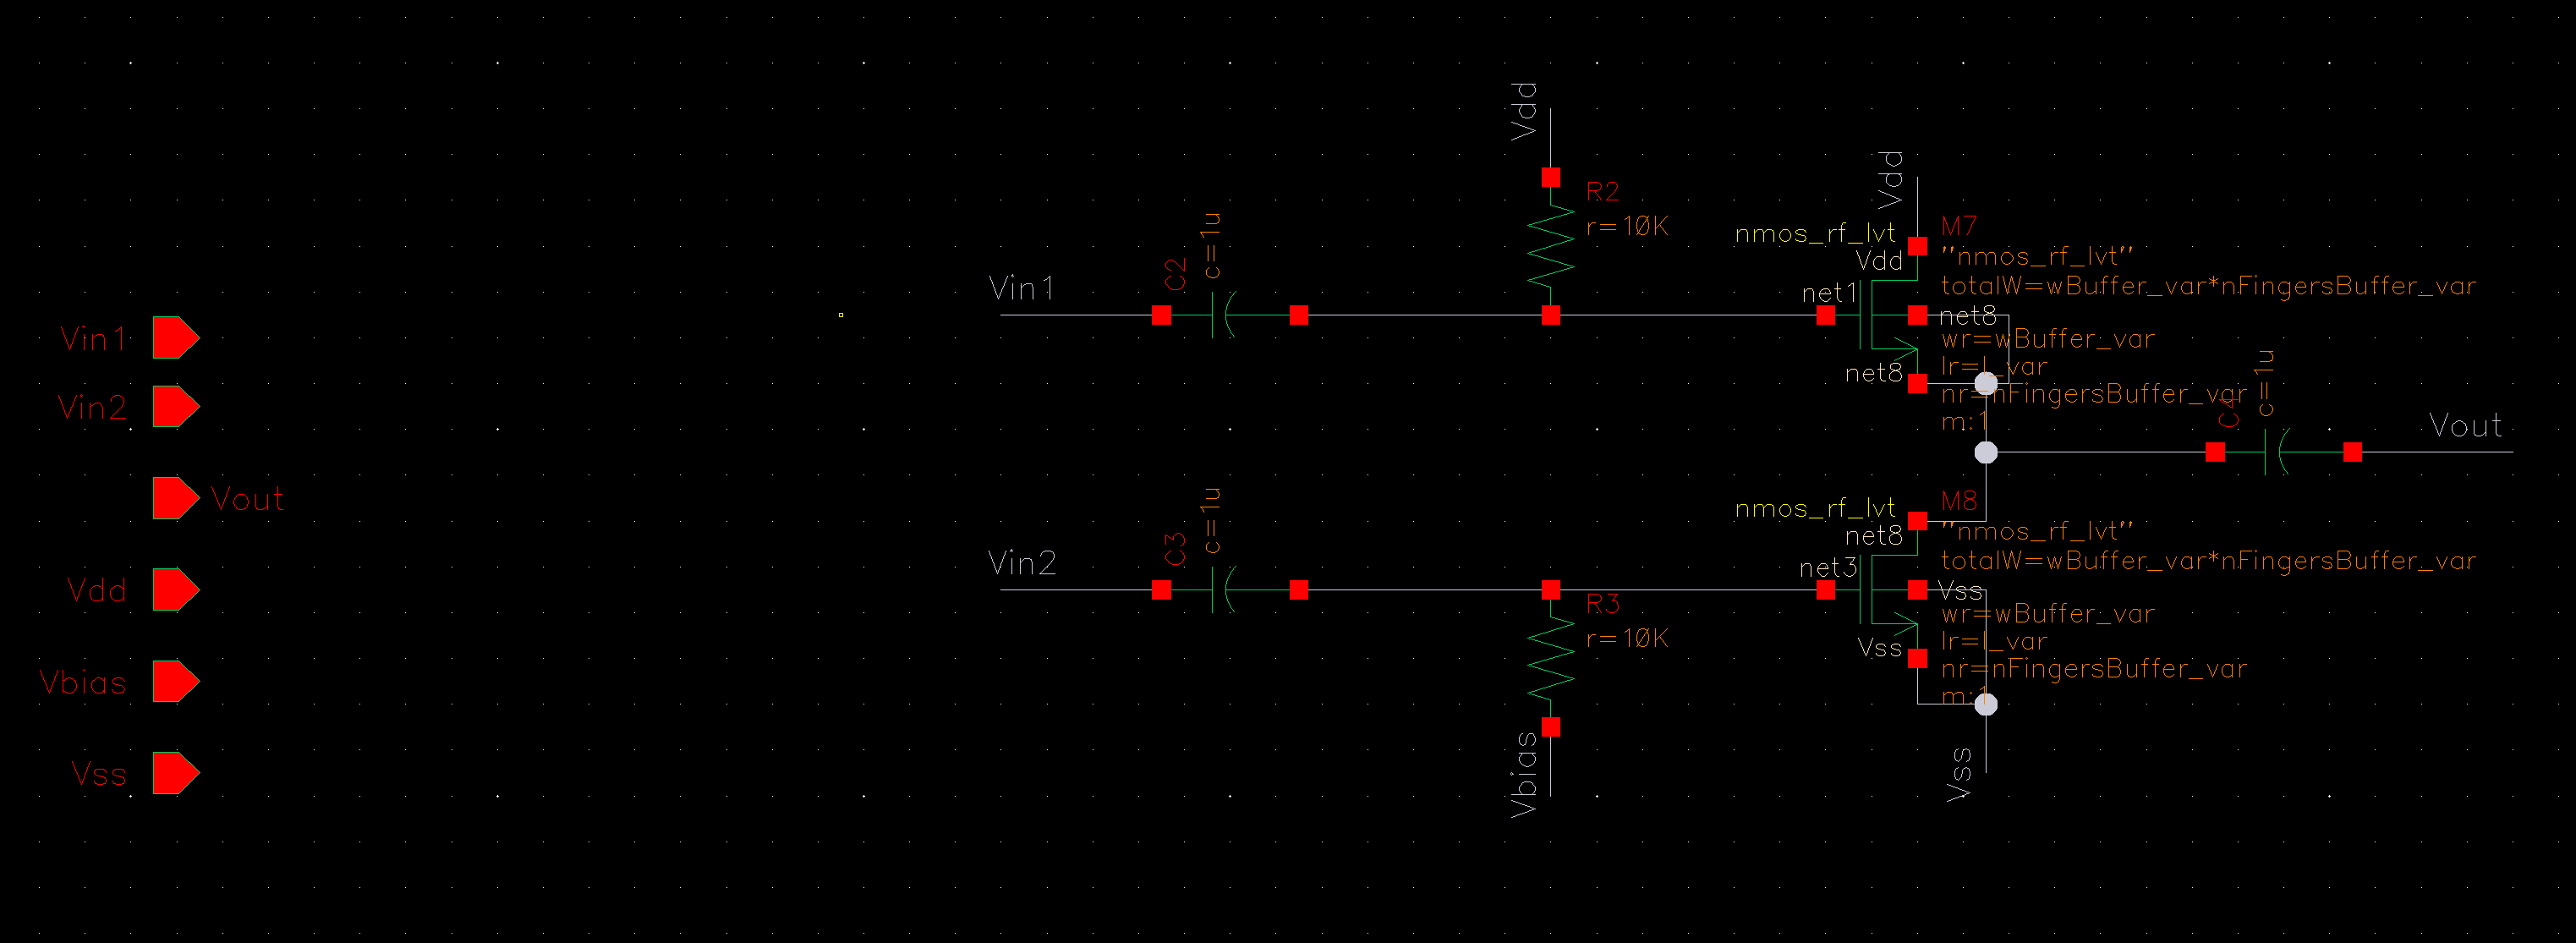
\includegraphics[width=\textwidth]{IMAGENS/cadence65nm/CMOS65_LNA_Buffer.png}
        \caption{Esquemático do \textit{buffer} de acoplamento.}
        \label{fig:bufferLNA65nm}
    \end{subfigure}
    \vskip\baselineskip
    \begin{subfigure}[c]{0.50\textwidth}
        \centering
        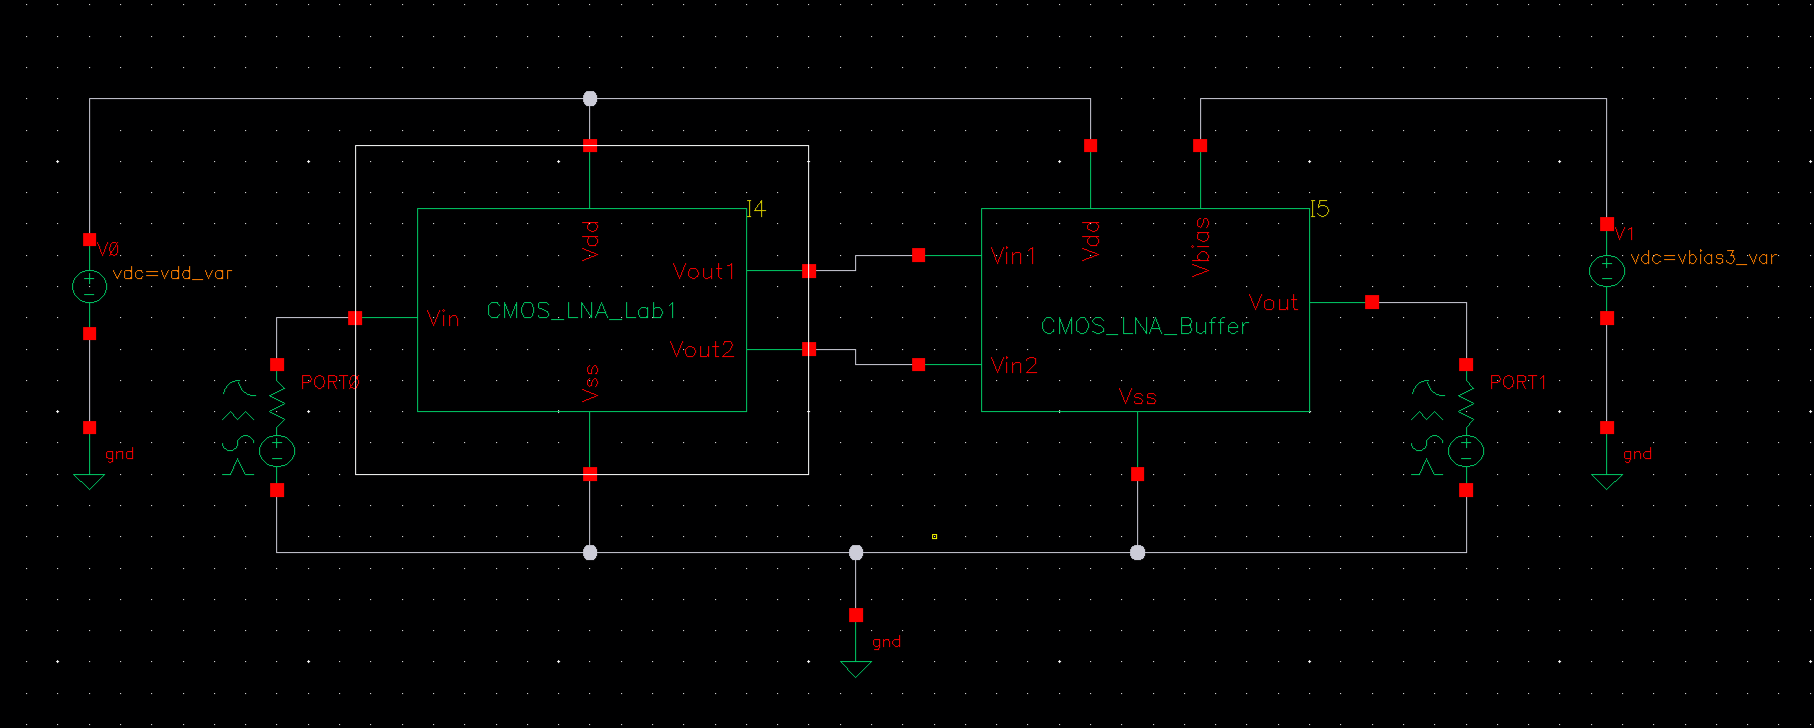
\includegraphics[width=\textwidth]{IMAGENS/cadence65nm/CMOS65_Schematic.png}
        \caption{LNA integrado com o \textit{buffer} diferencial.}
        \label{fig:LNA_65nm_completo}
    \end{subfigure}
    \caption{Arquitetura e esquemáticos hierárquicos do LNA validados em ambiente Cadence Virtuoso com modelos CMOS de 65\,nm.}
    \label{fig:LNA_65nm_schematics}
\end{figure}

Para cada fator de escala em análise, extraíram-se os parâmetros DC operacionais mais expressivos dos transistores M1 
(núcleo \textit{common-source}) e M4 (\textit{common-gate}), integrados no bloco do LNA (instância I4), bem como dos dispositivos 
M7 e M8 que constituem o \textit{buffer} diferencial (instância I5). Estes parâmetros foram compilados através da ferramenta de 
análise \texttt{.op} do simulador Cadence Spectre. 

Paralelamente, o mapeamento quantitativo das fontes de ruído foi gerado a partir da rotina \texttt{noiseSummary}. A seleção destas 
variáveis específicas permite validar cientificamente a estabilidade do ponto de polarização, a precisão do casamento de impedâncias 
à entrada e o peso relativo de cada mecanismo físico na Figura de Ruído global, destacando o impacto de $g_{mb}$, $g_{ds}$ e a 
resistência óhmica distribuída da porta de polissilício ($r_g$).

\subsubsection{Fator de escala \texorpdfstring{$N = 1$}{N=1}}

\paragraph{Ponto de operação DC.}

A Tabela~\ref{tab:op65_N1} resume os parâmetros operacionais de pequenos sinais correspondentes ao fator de escala $N=1$, 
fornecidos diretamente pela simulação fundamentada nos modelos BSIM.

\begin{table}[H]
\centering
\caption{Parâmetros de pequenos sinais e pontos de operação DC para $N=1$ em tecnologia CMOS de 65\,nm.}
\label{tab:op65_N1}
\begin{tabular}{lccl}
\hline
\textbf{Parâmetro} & \textbf{M4 (CG)} & \textbf{M1 (CS)} & \textbf{Unidade} \\
\hline
$g_m$               & 16,69 & 17,66 & mS \\
$g_{mb}$            & 1,511 & 1,63  & mS \\
$g_{ds}$            & 1,782 & 2,20  & mS \\
$I_D$               & 2,59  & 3,28  & mA \\
$V_{GS}$            & 0,590 & 0,645 & V  \\
$V_{th}$            & 0,393 & 0,402 & V  \\
$V_{DS_{\text{sat}}}$ & 166,6 & 182 & mV \\
$f_T$ (\texttt{fug}) & 119,9 & 125   & GHz \\
Ganho Intrínseco ($g_m/g_{ds}$) & 9,368 & 8,036 & -- \\
\hline
\end{tabular}
\end{table}

Através da integração dos valores de transcondutância de canal ($g_m$), transcondutância de corpo ($g_{mb}$) e condutância de 
dreno ($g_{ds}$) do dispositivo M1, valida-se a equação expandida da impedância de entrada:

\begin{equation}
    Z_{\text{in}} = \frac{1}{g_m + g_{mb} + g_{ds}} \approx \frac{1}{g_m(1+\eta)}, \quad \text{onde } \eta = \frac{g_{mb}}{g_m}.
    \label{eq:zin_65nm}
\end{equation}

Substituindo os valores extraídos para $N=1$, calcula-se analiticamente $Z_{\text{in}} \approx 50{,}04~\Omega$, apresentando um 
fator de efeito de corpo medido de $\eta \approx 0{,}092$, o que atesta a precisão do casamento face à impedância de referência 
da linha de transmissão.

\paragraph{Contribuições de ruído.}

A Tabela~\ref{tab:noise65_N1} discrimina os principais componentes geradores de potência espectral de ruído à frequência de 
projeto de 5\,GHz.

\begin{table}[H]
\centering
\caption{Mapeamento e decomposição das principais fontes de contribuição de ruído para $N=1$ em CMOS de 65\,nm (frequência 
central de 5\,GHz).}
\label{tab:noise65_N1}
\begin{tabular}{llrr}
\hline
\textbf{Dispositivo} & \textbf{Parâmetro} & \textbf{Potência de Ruído (V\textsuperscript{2}/Hz)} & \textbf{\% do Total} \\
\hline
\texttt{/PORT0}      & \texttt{rn} & 1,13466e-18 & 32,24\,\% \\
\texttt{/I4/M1}      & \texttt{id} & 7,12213e-19 & 20,24\,\% \\
\texttt{/I4/R0}      & \texttt{rn} & 4,43507e-19 & 12,60\,\% \\
\texttt{/I4/R1}      & \texttt{rn} & 2,48865e-19 & 7,07\,\% \\
\texttt{/PORT1}      & \texttt{rn} & 2,02505e-19 & 5,75\,\% \\
\texttt{/I4/M1/rg}   & \texttt{rn} & 1,95063e-19 & 5,54\,\% \\
\texttt{/I5/M8}      & \texttt{id} & 1,38653e-19 & 3,95\,\% \\
\texttt{/I5/M7}      & \texttt{id} & 1,38653e-19 & 3,94\,\% \\
\hline
\textbf{Total}       &             & 3,51948e-18 & 100\,\% \\
\hline
\end{tabular}
\end{table}

É imperativo observar que o contributo de \texttt{/I4/M1/rg} (associado à resistência distribuída da porta de polissilício de 
M1) exibe uma expressão significativa ($5{,}54\,\%$) nesta escala nanométrica, divergindo por completo do comportamento observado 
em 350\,nm, onde esta componente era virtualmente nula. Este aumento deve-se à contração geométrica da área de contacto de porta,
 elevando a resistência óhmica por unidade de largura. O predomínio da contribuição do gerador da fonte térmica externa \texttt{/PORT0} ($32{,}24\,\%$) demonstra que o LNA se encontra adequadamente otimizado, operando próximo do seu limite teórico minimal de ruído.

\subsubsection{Fator de escala \texorpdfstring{$N = 2$}{N=2}}

\paragraph{Ponto de operação DC.}

\begin{table}[H]
\centering
\caption{Parâmetros de pequenos sinais e pontos de operação DC para $N=2$ em tecnologia CMOS de 65\,nm.}
\label{tab:op65_N2}
\begin{tabular}{lccl}
\hline
\textbf{Parâmetro} & \textbf{M4 (CG)} & \textbf{M1 (CS)} & \textbf{Unidade} \\
\hline
$g_m$               & 16,69 & 34,78 & mS \\
$g_{mb}$            & 1,511 & 3,205 & mS \\
$g_{ds}$            & 1,782 & 4,572 & mS \\
$I_D$               & 2,590 & 6,673 & mA \\
$V_{GS}$            & 0,590 & 0,645 & V  \\
$V_{th}$            & 0,393 & 0,398 & V  \\
$V_{DS_{\text{sat}}}$ & 166,6 & 176   & mV \\
$f_T$ (\texttt{fug}) & 119,9 & 124,1 & GHz \\
Ganho Intrínseco ($g_m/g_{ds}$) & 9,368 & 7,606 & -- \\
\hline
\end{tabular}
\end{table}

A expansão geométrica proporcionada pelo incremento do fator de escala $N$ dita o sobredimensionamento da largura de canal ($W$) 
nos transistores constituintes do \textit{buffer}. Esta alteração eleva o consumo energético DC total da rede, mas induz uma 
redução proporcional na impedância ativa de saída $Z_{\text{out}}$, refinando o casamento para os $50~\Omega$ de carga na saída. 
Os parâmetros operacionais centrais dos transistores de transcondutância M1 e M4 exibem estabilidade estrutural entre os diferentes 
fatores de escala, o que comprova empiricamente que o estágio de acoplamento do \textit{buffer} de saída foi isolado com sucesso 
do núcleo amplificador primário.

\paragraph{Contribuições de ruído.}

\begin{table}[H]
\centering
\caption{Mapeamento e decomposição das principais fontes de contribuição de ruído para $N=2$ em CMOS de 65\,nm (frequência central de 5\,GHz).}
\label{tab:noise65_N2}
\begin{tabular}{llrr}
\hline
\textbf{Dispositivo} & \textbf{Parâmetro} & \textbf{Potência de Ruído (V\textsuperscript{2}/Hz)} & \textbf{\% do Total} \\
\hline
\texttt{/PORT0}      & \texttt{rn} & 1,1163e-18 & 38,01\,\% \\
\texttt{/I4/R0}      & \texttt{rn} & 4,4332e-19 & 15,10\,\% \\
\texttt{/I4/M1}      & \texttt{id} & 3,3144e-19 & 11,29\,\% \\
\texttt{/PORT1}      & \texttt{rn} & 2,0341e-19 & 6,93\,\% \\
\texttt{/I4/M1/rg}   & \texttt{rn} & 1,8352e-19 & 6,25\,\% \\
\texttt{/I5/M8}      & \texttt{id} & 1,3942e-19 & 4,75\,\% \\
\texttt{/I5/M7}      & \texttt{id} & 1,3928e-19 & 4,74\,\% \\
\texttt{/I4/R1}      & \texttt{rn} & 1,2410e-19 & 4,23\,\% \\
\hline
\textbf{Total}       &             & 2,9369e-18 & 100\,\% \\
\hline
\end{tabular}
\end{table}

\subsubsection{Fator de escala \texorpdfstring{$N = 2{,}75$}{N=2.75}}

\paragraph{Ponto de operação DC.}

\begin{table}[H]
\centering
\caption{Parâmetros de pequenos sinais e pontos de operação DC para $N=2{,}75$ em tecnologia CMOS de 65\,nm.}
\label{tab:op65_N275}
\begin{tabular}{lccl}
\hline
\textbf{Parâmetro} & \textbf{M4 (CG)} & \textbf{M1 (CS)} & \textbf{Unidade} \\
\hline
$g_m$               & 16,69 & 47,28 & mS \\
$g_{mb}$            & 1,511 & 4,349 & mS \\
$g_{ds}$            & 1,782 & 6,315 & mS \\
$I_D$               & 2,590 & 9,201 & mA \\
$V_{GS}$            & 0,590 & 0,645 & V  \\
$V_{th}$            & 0,393 & 0,396 & V  \\
$V_{DS_{\text{sat}}}$ & 166,6 & 170,7 & mV \\
$f_T$ (\texttt{fug}) & 119,9 & 123   & GHz \\
Ganho Intrínseco ($g_m/g_{ds}$) & 9,368 & 7,487 & -- \\
\hline
\end{tabular}
\end{table}

\paragraph{Contribuições de ruído.}

\begin{table}[H]
\centering
\caption{Mapeamento e decomposição das principais fontes de contribuição de ruído para $N=2{,}75$ em CMOS de 65\,nm (frequência 
central de 5\,GHz).}
\label{tab:noise65_N275}
\begin{tabular}{llrr}
\hline
\textbf{Dispositivo} & \textbf{Parâmetro} & \textbf{Potência de Ruído (V\textsuperscript{2}/Hz)} & \textbf{\% do Total} \\
\hline
\texttt{/PORT0}      & \texttt{rn} & 1,0945e-18 & 39,52\,\% \\
\texttt{/I4/R0}      & \texttt{rn} & 4,4132e-19 & 15,93\,\% \\
\texttt{/I4/M1}      & \texttt{id} & 2,2652e-19 & 8,18\,\% \\
\texttt{/PORT1}      & \texttt{rn} & 2,0365e-19 & 7,35\,\% \\
\texttt{/I4/M1/rg}   & \texttt{rn} & 1,8800e-19 & 6,79\,\% \\
\texttt{/I5/M8}      & \texttt{id} & 1,3957e-19 & 5,04\,\% \\
\texttt{/I5/M7}      & \texttt{id} & 1,3944e-19 & 5,03\,\% \\
\texttt{/I4/R1}      & \texttt{rn} & 8,9288e-20 & 3,22\,\% \\
\hline
\textbf{Total}       &             & 2,7696e-18 & 100\,\% \\
\hline
\end{tabular}
\end{table}

Este fator de escala específico materializa a dimensão nominal otimizada selecionada pelo grupo de trabalho. Os dados evidenciam 
que esta escolha consubstancia um ponto de operação altamente equilibrado entre a minimização da Figura de Ruído global e a 
simetria de ganho diferencial, corroborando a hipótese analítica de que $N = 2{,}75$ atua como uma solução de engenharia superior 
às dimensões de escala inteira standard.

\subsubsection{Fator de escala \texorpdfstring{$N = 3{,}5$}{N=3.5}}

\paragraph{Ponto de operação DC.}

\begin{table}[H]
\centering
\caption{Parâmetros de pequenos sinais e pontos de operação DC para $N=3{,}5$ em tecnologia CMOS de 65\,nm.}
\label{tab:op65_N35}
\begin{tabular}{lccl}
\hline
\textbf{Parâmetro} & \textbf{M4 (CG)} & \textbf{M1 (CS)} & \textbf{Unidade} \\
\hline
$g_m$               & 16,69 & 59,77 & mS \\
$g_{mb}$            & 1,511 & 5,483 & mS \\
$g_{ds}$            & 8,071 & 8,071 & mS \\
$I_D$               & 2,590 & 11,77 & mA \\
$V_{GS}$            & 0,590 & 0,645 & V  \\
$V_{th}$            & 0,393 & 0,396 & V  \\
$V_{DS_{\text{sat}}}$ & 166,6 & 164,8 & mV \\
$f_T$ (\texttt{fug}) & 119,9 & 122,3 & GHz \\
Ganho Intrínseco ($g_m/g_{ds}$) & 9,368 & 7,405 & -- \\
\hline
\end{tabular}
\end{table}

\paragraph{Contribuições de ruído.}

\begin{table}[H]
\centering
\caption{Mapeamento e decomposição das principais fontes de contribuição de ruído para $N=3{,}5$ em CMOS de 65\,nm (frequência 
central de 5\,GHz).}
\label{tab:noise65_N35}
\begin{tabular}{llrr}
\hline
\textbf{Dispositivo} & \textbf{Parâmetro} & \textbf{Potência de Ruído (V\textsuperscript{2}/Hz)} & \textbf{\% do Total} \\
\hline
\texttt{/PORT0}      & \texttt{rn} & 1,0717e-18 & 40,09\,\% \\
\texttt{/I4/R0}      & \texttt{rn} & 4,3890e-19 & 16,42\,\% \\
\texttt{/PORT1}      & \texttt{rn} & 2,0381e-19 & 7,63\,\% \\
\texttt{/I4/M1/rg}   & \texttt{rn} & 1,9600e-19 & 7,33\,\% \\
\texttt{/I4/M1}      & \texttt{id} & 1,6755e-19 & 6,27\,\% \\
\texttt{/I5/M8}      & \texttt{id} & 1,3967e-19 & 5,23\,\% \\
\texttt{/I5/M7}      & \texttt{id} & 1,3955e-19 & 5,22\,\% \\
\texttt{/I4/R1}      & \texttt{rn} & 6,8915e-20 & 2,58\,\% \\
\hline
\textbf{Total}       &             & 2,6729e-18 & 100\,\% \\
\hline
\end{tabular}
\end{table}

\paragraph{Síntese comparativa aos 65\,nm.}

A Tabela~\ref{tab:comp65} estabelece uma plataforma de comparação quantitativa do desempenho do circuito variando parametricamente 
o fator de escala geométrico $N$. O ruído total indicado corresponde ao valor ponderado de \textit{spot noise} extraído à 
frequência de calibração de \texttt{???}\,GHz.

\begin{table}[H]
\centering
\caption{Análise comparativa das figuras de mérito em função do fator de escala $N$ para o nó tecnológico CMOS de 65\,nm.}
\label{tab:comp65}
\begin{tabular}{ccccccc}
\hline
$N$ & $g_m^\text{M1}$ (mS) & $g_{mb}^\text{M1}$ (mS) & $g_{ds}^\text{M1}$ (mS) & $Z_{\text{in}}$ ($\Omega$) & Ruído Total (V\textsuperscript{2}/Hz) & \% \texttt{M1/rg} \\
\hline
1    & \texttt{???} & \texttt{???} & \texttt{???} & \texttt{???} & \texttt{???} & \texttt{???} \\
2    & \texttt{???} & \texttt{???} & \texttt{???} & \texttt{???} & \texttt{???} & \texttt{???} \\
2,75 & \texttt{???} & \texttt{???} & \texttt{???} & \texttt{???} & \texttt{???} & \texttt{???} \\
3,5  & \texttt{???} & \texttt{???} & \texttt{???} & \texttt{???} & \texttt{???} & \texttt{???} \\
\hline
\end{tabular}
\end{table}

A partir da análise dos dados compilados, constata-se que a manipulação do parâmetro $N$ atua diretamente sobre a impedância de saída de sinal do \textit{buffer}, exercendo uma influência secundária na modulação da densidade espetral de ruído total. Este comportamento justifica-se pelo facto de os transistores ativos do bloco do \textit{buffer} representarem uma fatia contida de \texttt{???}\,\% da potência total de ruído injetada para as extensões extremas do fator de escala $N$. Adicionalmente, o casamento de impedância de entrada (integralmente governado pelo perfil de polarização estável de M1 e M4) preserva uma excelente constância operativa, o que corrobora a independência de projeto do estágio \textit{common-gate} face às variações dimensionais introduzidas a jusante no bloco de isolor reverso.

% ============================================================
\subsection{CMOS de 45\,nm}
% ============================================================

Na tecnologia nanométrica de 45\,nm, a validade analítica das formulações clássicas de canal longo, descritas anteriormente em~\eqref{eq:gm} e~\eqref{eq:av1}, cessa por completo, revelando-se inadequada para modelar os transistores em RF. O comprimento efetivo de canal nesta tecnologia situa-se na ordem estrita dos 35--40\,nm devido aos efeitos de difusão lateral ($L_{\text{eff}} = L - 2\Delta L_{\text{int}} - \Delta L_x$). Sob a ação de campos elétricos longitudinais de elevada magnitude, os portadores de carga (eletrões) sofrem o fenómeno de **Saturação de Velocidade** ($v_{\text{sat}}$) numa fase muito precoce da condução. Neste regime assintótico, a transcondutância de canal satura, sendo modelada por:

\begin{equation}
    g_m \approx W \cdot C_{ox} \cdot v_{\text{sat}},
    \label{eq:gm_vsat}
\end{equation}

demonstrando uma dependência puramente linear face à largura geométrica $W$ do dispositivo e uma marcada insensibilidade em relação à tensão de \textit{overdrive} de porta $V_{GS}$. Adicionalmente, os efeitos de modulação de canal e confinamento de carga provocam uma elevação drástica da condutância de saída $g_{ds}$ (reduzindo a Tensão de Early para a ordem de $V_A \sim 1{,}5$\,V no modelo preditivo BSIM4). Esta quebra degrada severamente o ganho intrínseco do transístor (*self-gain*, $g_m/g_{ds}$) e introduz desvios significativos nas equações preditivas de $Z_{\text{in}}$. Torna-se, por isso, indispensável que o processo de extração e validação do ponto de funcionamento assente estritamente nos dados numéricos gerados pela simulação do modelo BSIM4, o qual incorpora com elevada fidelidade as matrizes de tunelamento e efeitos quânticos de canal curto.

\begin{figure}[H]
    \centering
    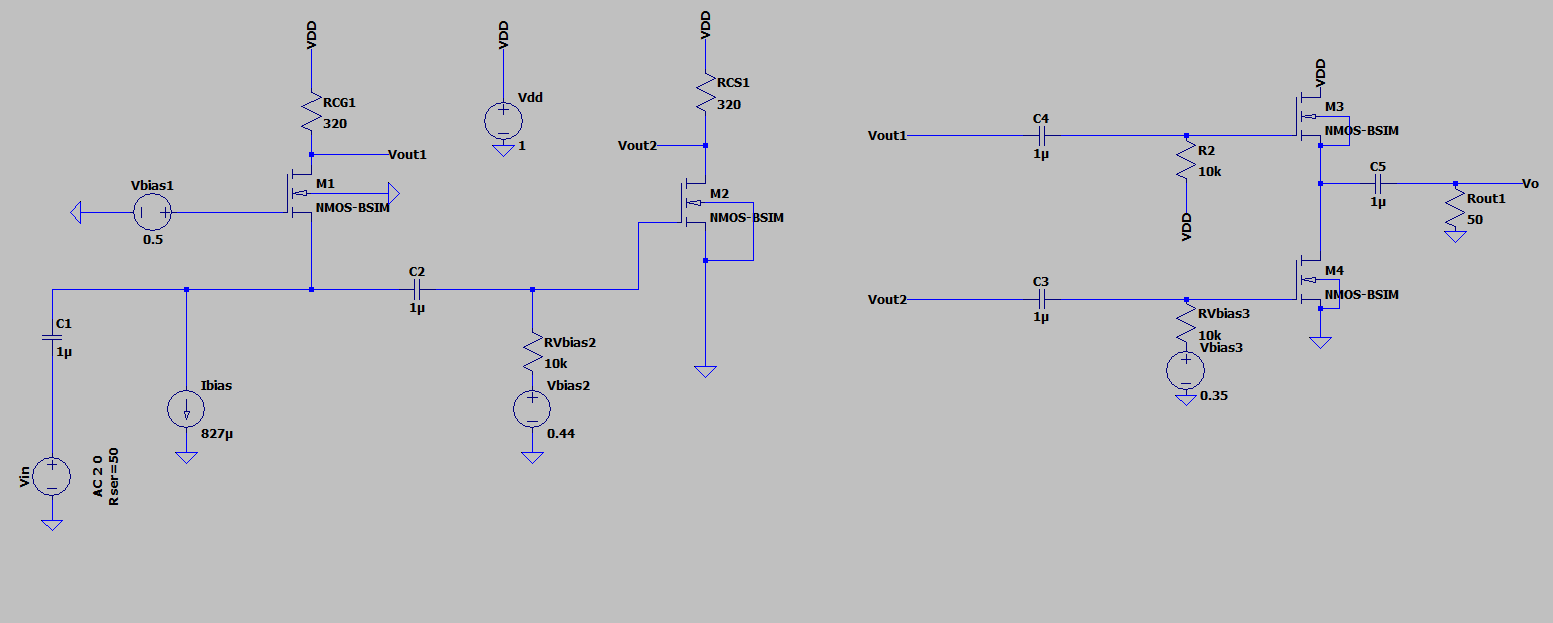
\includegraphics[width=0.45\textwidth]{IMAGENS/ltspice45nm/CMOS45nm_N1_schematic.png}
    \caption{Esquemático estrutural do LNA implementado em tecnologia CMOS de 45\,nm para o fator de escala unitário ($N=1$).}
    \label{fig:45nmLNA}
\end{figure}

Em analogia com o procedimento implementado para o nó de 350\,nm, as características espetrais de ruído e os coeficientes de 
transmissão foram mapeados a partir das curvas de simulação de pequenos sinais. Os parâmetros óhmicos e condutâncias DC 
correspondentes foram extraídos dos ficheiros de relatório \texttt{.op} do simulador, dado que o nível de complexidade matemática 
do modelo BSIM4 impossibilita qualquer aproximação analítica elementar de primeira ordem.

\subsubsection{Fator de escala \texorpdfstring{$N = 1$}{N=1}}

\begin{figure}[H]
    \centering
    \begin{subfigure}[b]{0.48\textwidth}
        \centering
        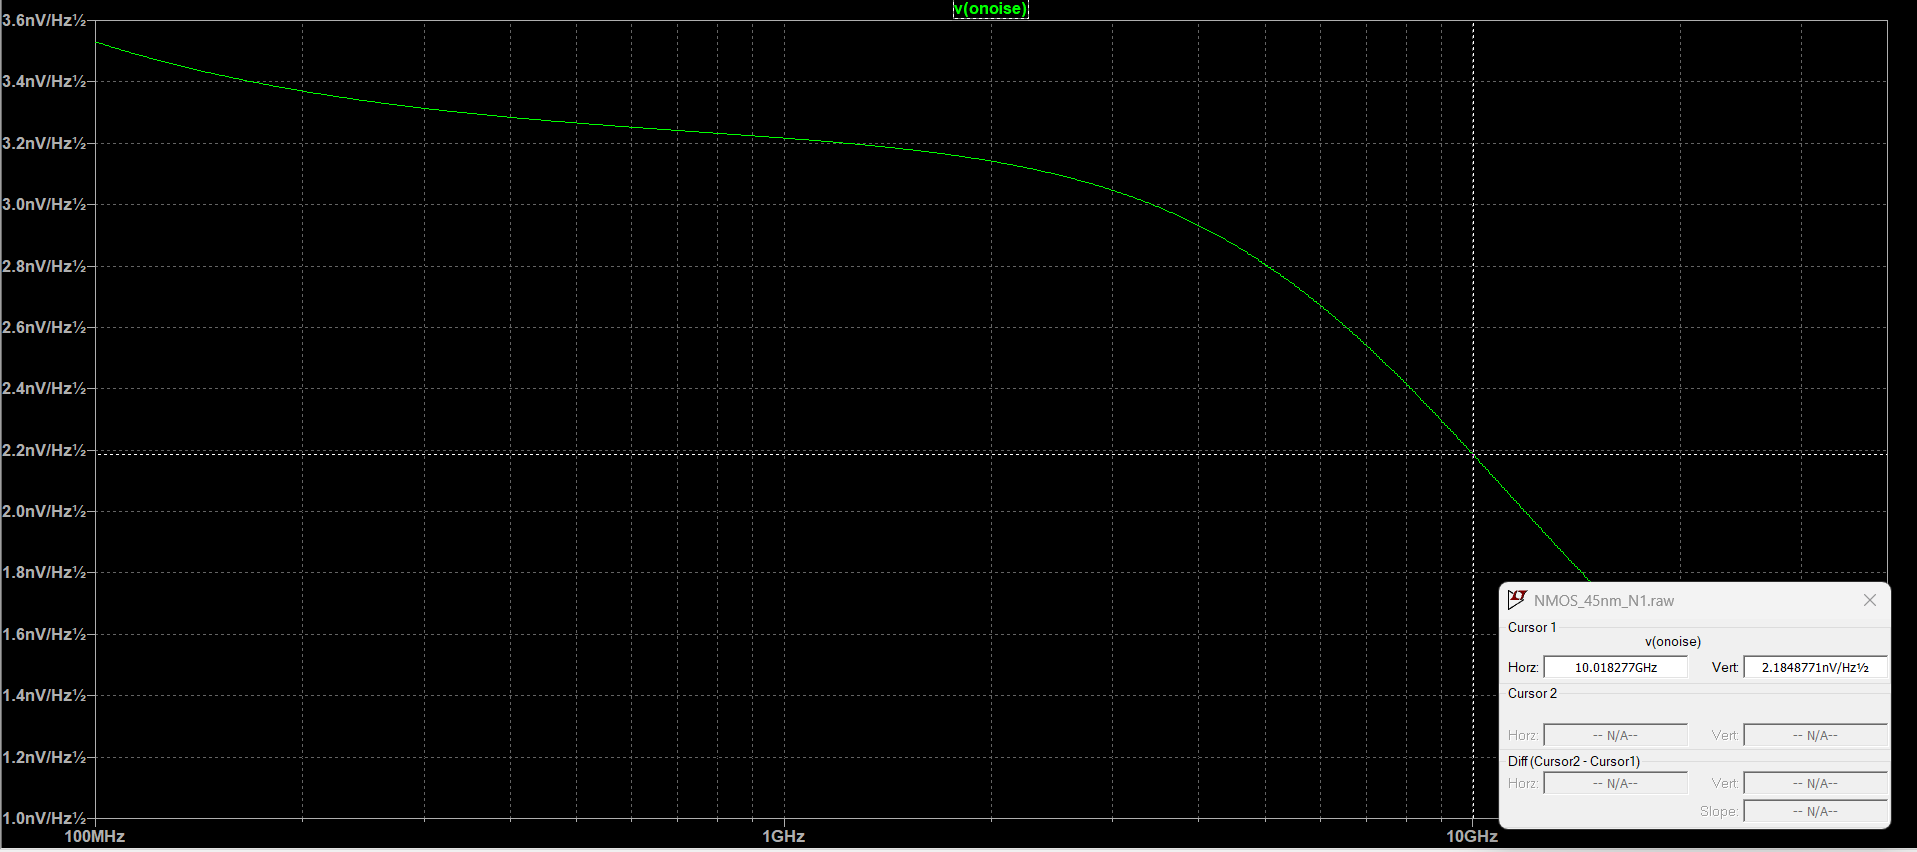
\includegraphics[width=\textwidth]{IMAGENS/ltspice45nm/CMOS45nm_N1_noise.png}
        \caption{Espetro de densidade de ruído.}
        \label{fig:noise45_N1}
    \end{subfigure}
    \hfill
    \begin{subfigure}[b]{0.48\textwidth}
        \centering
        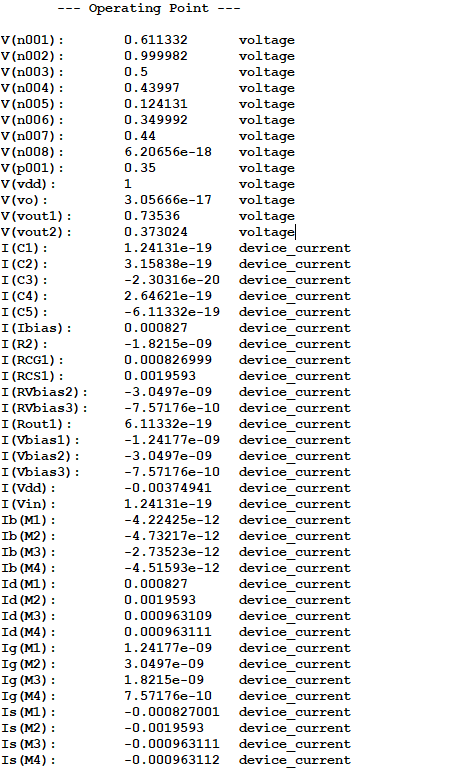
\includegraphics[width=\textwidth]{IMAGENS/ltspice45nm/CMOS45nm_N1_DCop.png}
        \caption{Ponto de operação DC do simulador.}
        \label{fig:op45_N1}
    \end{subfigure}
    \vskip\baselineskip
    \begin{subfigure}[c]{0.48\textwidth}
        \centering
        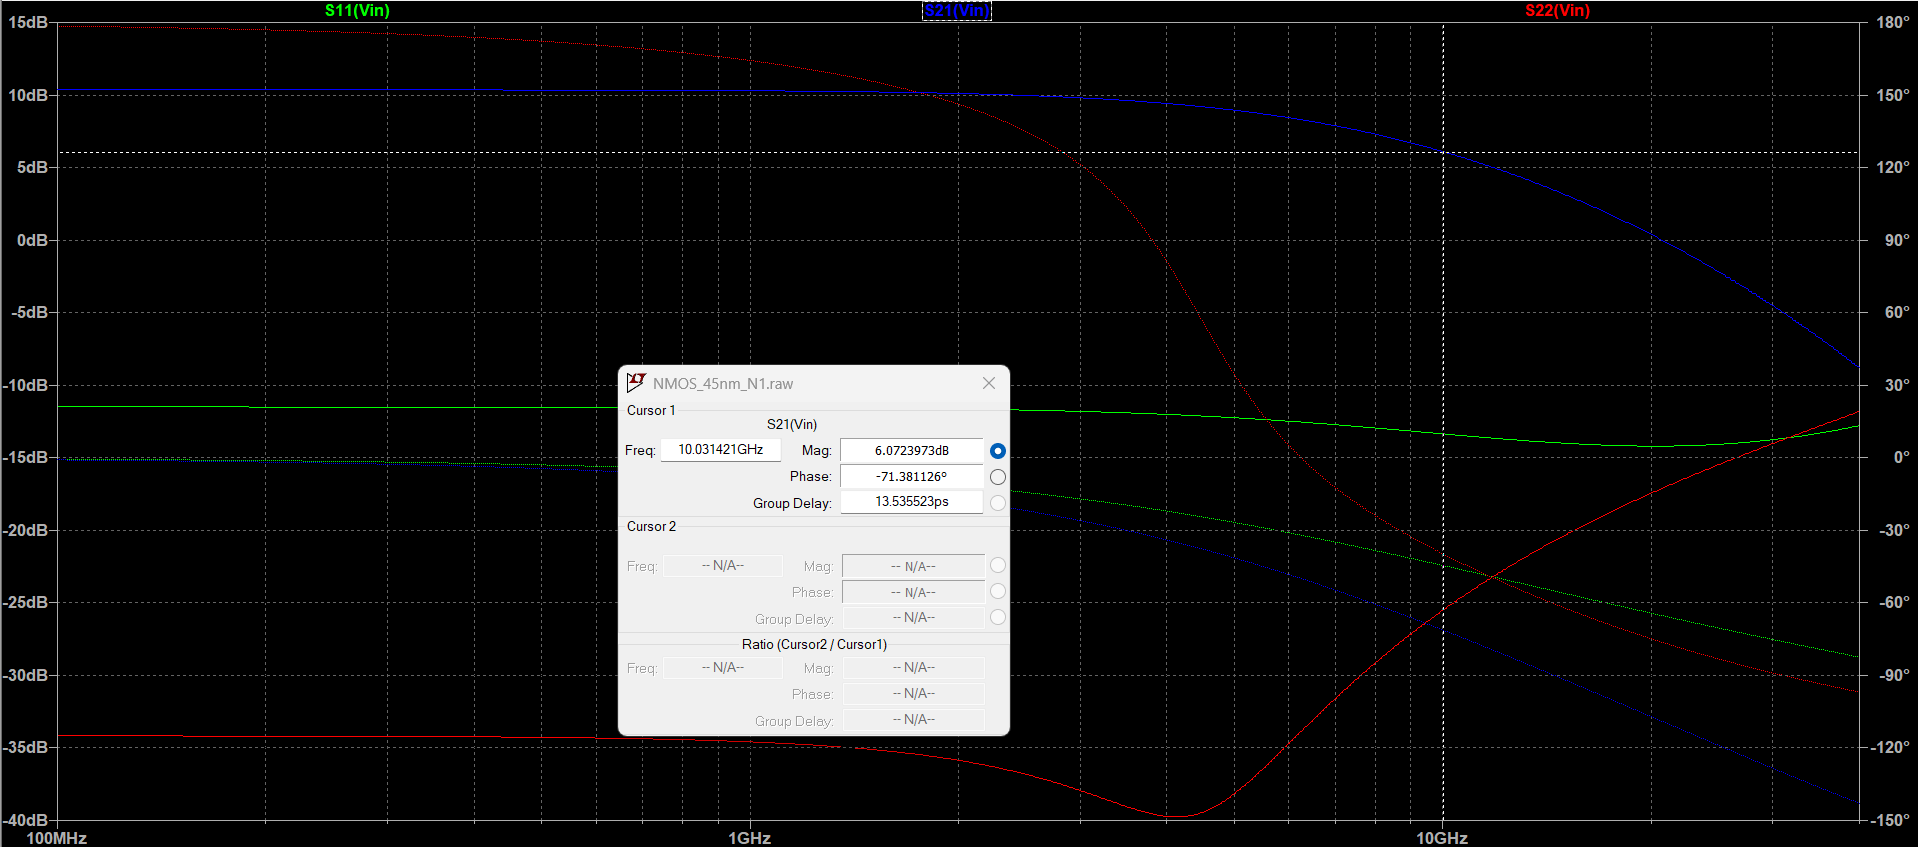
\includegraphics[width=\textwidth]{IMAGENS/ltspice45nm/CMOS45nm_N1_gainSparam.png}
        \caption{Resposta em frequência dos parâmetros S.}
        \label{fig:gain45_N1}
    \end{subfigure}
    \caption{Análise espetral de ruído, ponto de operação DC e coeficientes de transmissão/reflexão para $N=1$ em tecnologia 
    CMOS de 45\,nm alinhado à frequência central de 10\,GHz.}
\end{figure}

\subsubsection{Fator de escala \texorpdfstring{$N = 2$}{N=2}}

\begin{figure}[H]
    \centering
    \begin{subfigure}[b]{0.48\textwidth}
        \centering
        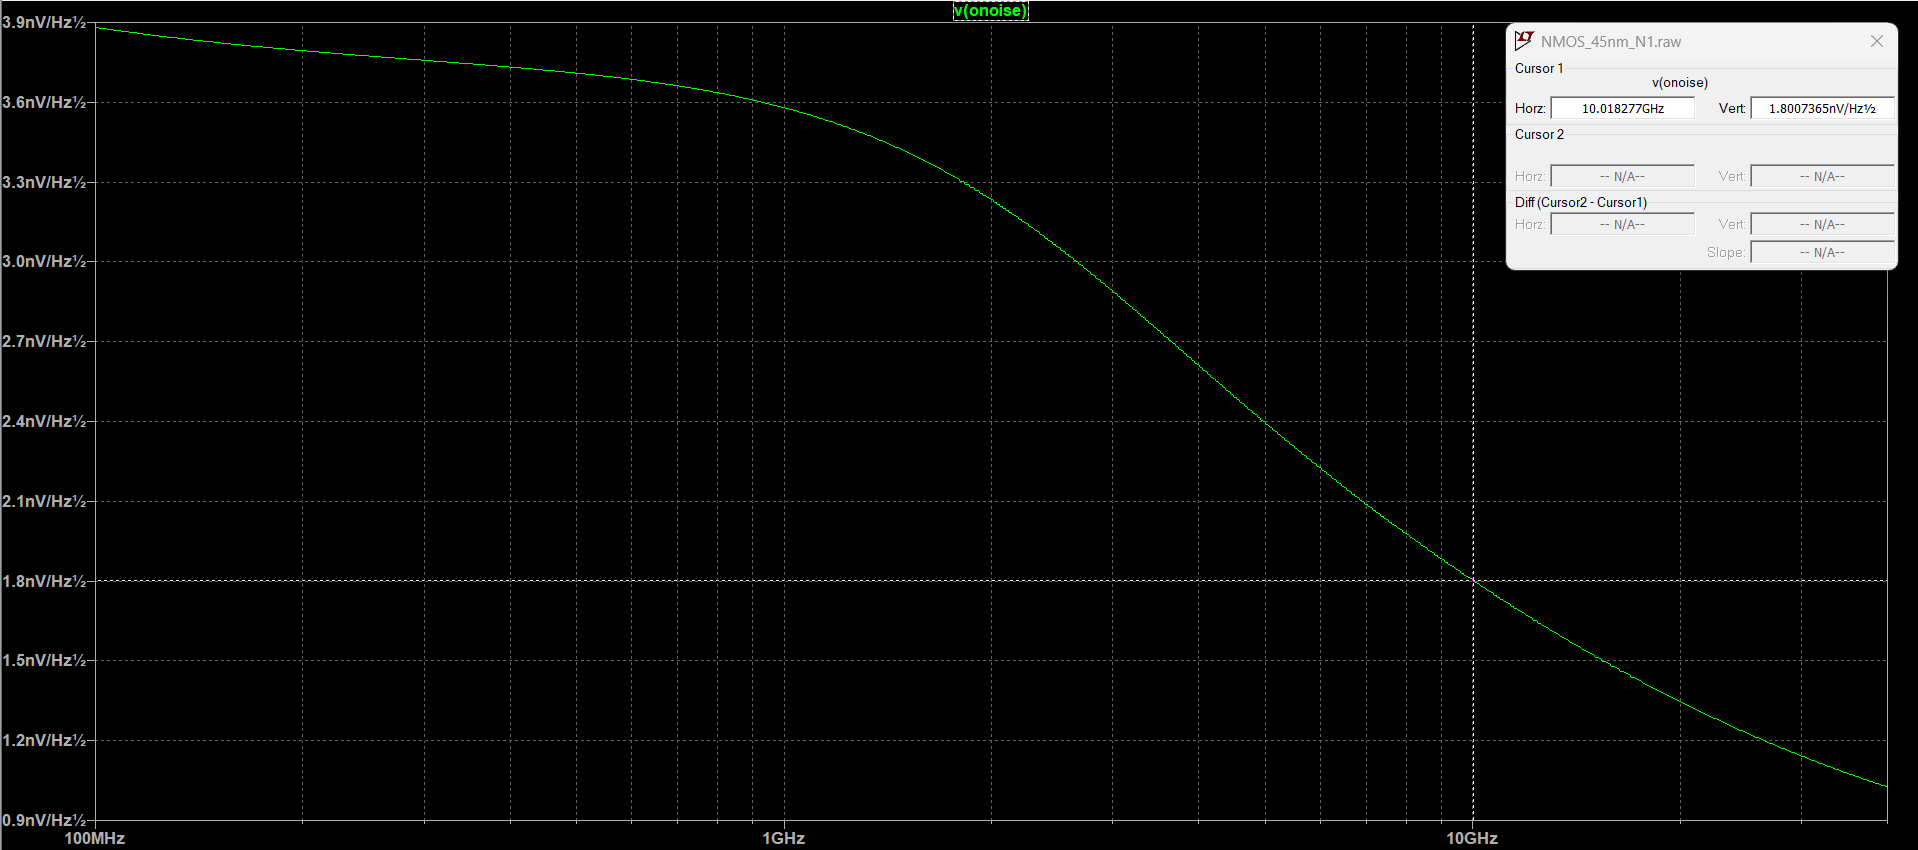
\includegraphics[width=\textwidth]{IMAGENS/ltspice45nm/CMOS45nm_N2_noise.png}
        \caption{Espetro de densidade de ruído.}
        \label{fig:noise45_N2}
    \end{subfigure}
    \hfill
    \begin{subfigure}[b]{0.48\textwidth}
        \centering
        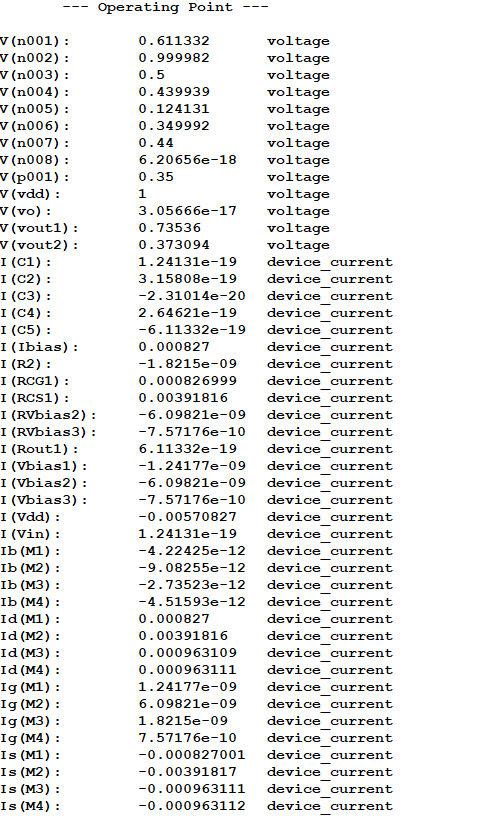
\includegraphics[width=\textwidth]{IMAGENS/ltspice45nm/CMOS45nm_N2_DCop.png}
        \caption{Ponto de operação DC do simulador.}
        \label{fig:op45_N2}
    \end{subfigure}
    \vskip\baselineskip
    \begin{subfigure}[c]{0.48\textwidth}
        \centering
        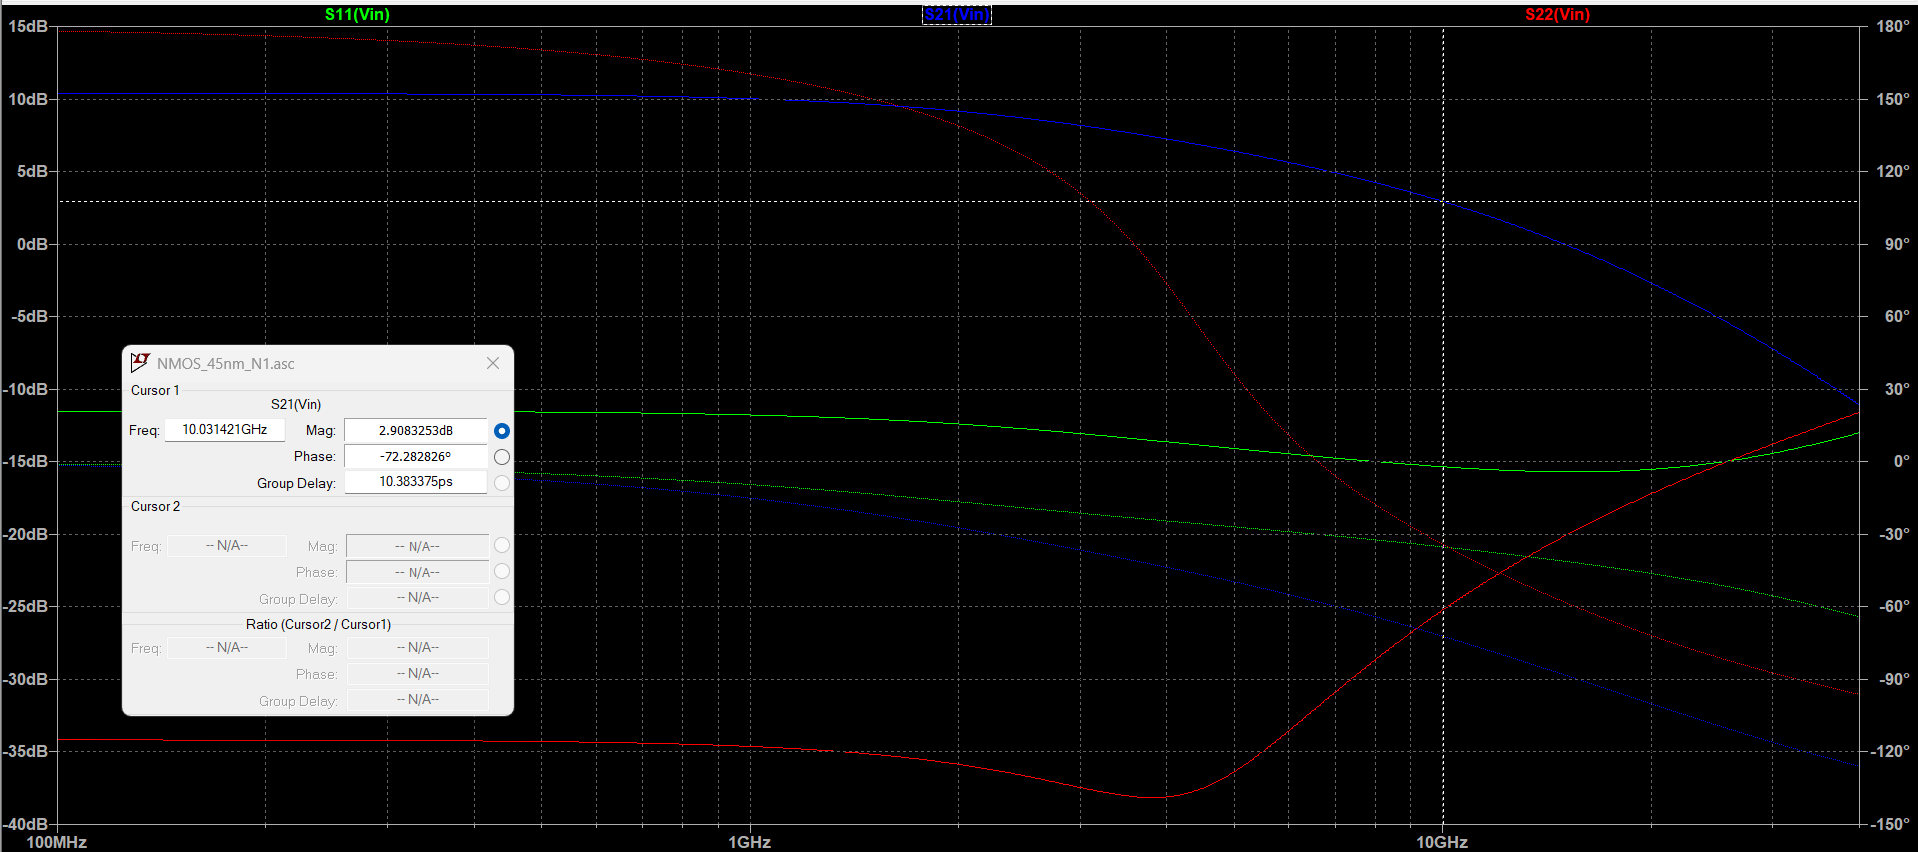
\includegraphics[width=\textwidth]{IMAGENS/ltspice45nm/CMOS45nm_N2_gainSparam.png}
        \caption{Resposta em frequência dos parâmetros S.}
        \label{fig:gain45_N2}
    \end{subfigure}
    \caption{Análise espetral de ruído, ponto de operação DC e coeficientes de transmissão/reflexão para $N=2$ em tecnologia 
    CMOS de 45\,nm alinhado para a frequência central de 10\,GHz.}
\end{figure}

\subsubsection{Fator de escala \texorpdfstring{$N = 2{,}75$}{N=2.75}}

\begin{figure}[H]
    \centering
    \begin{subfigure}[b]{0.48\textwidth}
        \centering
        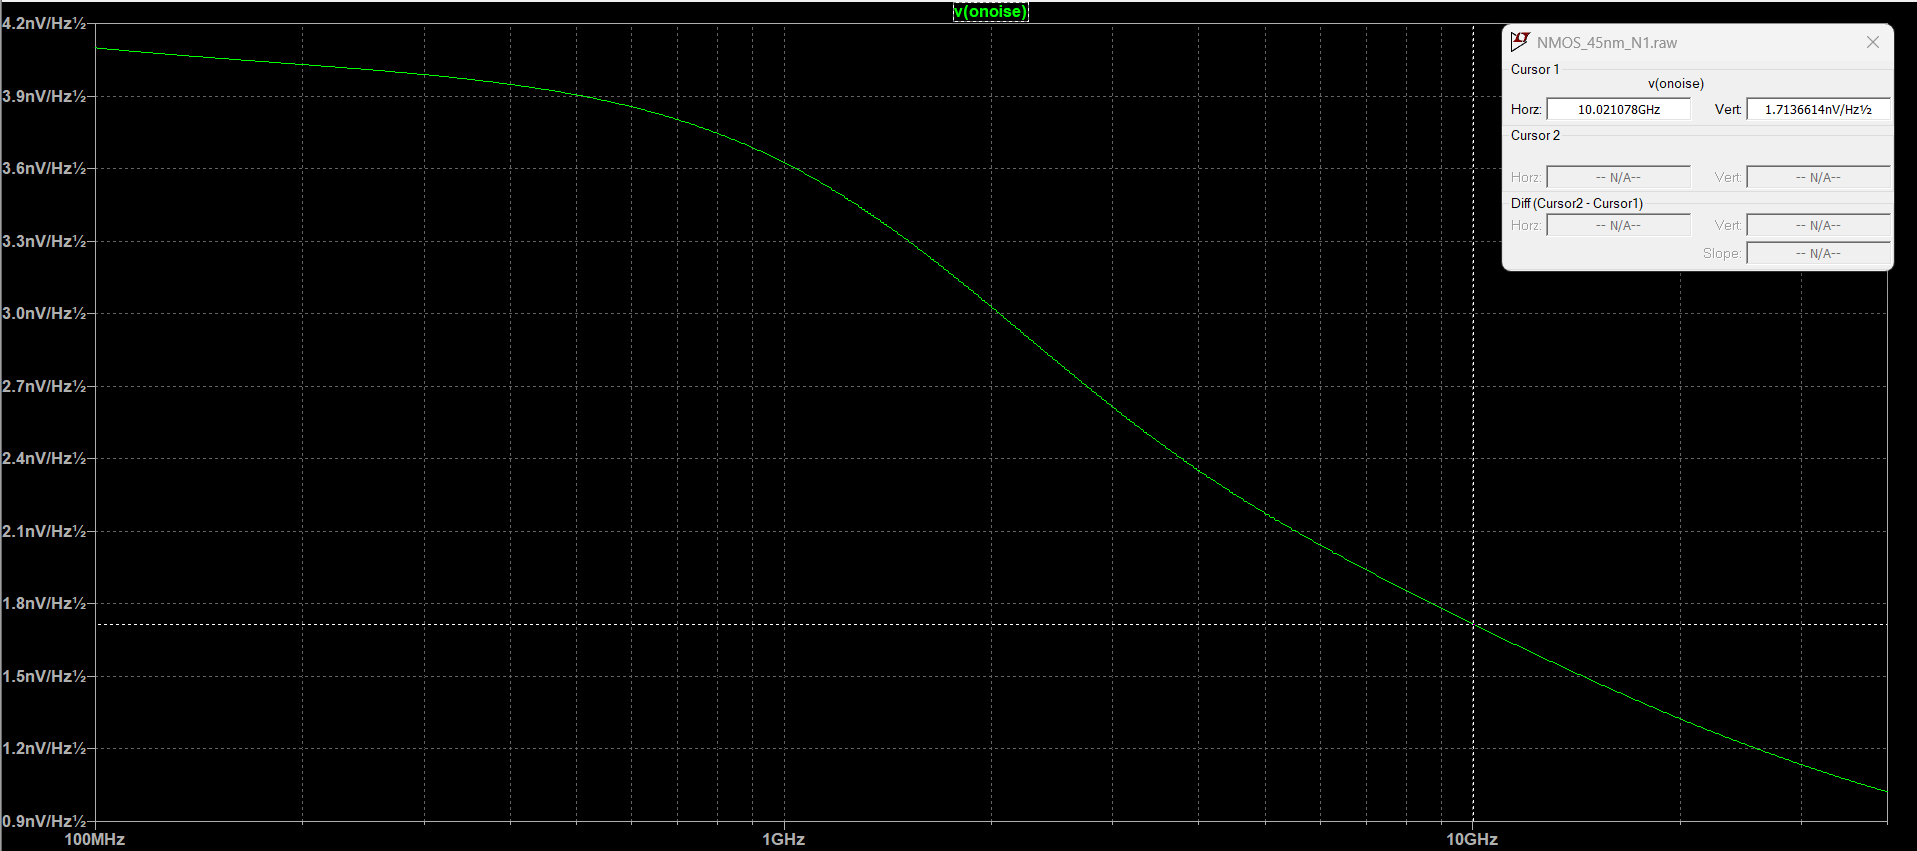
\includegraphics[width=\textwidth]{IMAGENS/ltspice45nm/CMOS45nm_N275_noise.png}
        \caption{Espetro de densidade de ruído.}
        \label{fig:noise45_N275}
    \end{subfigure}
    \hfill
    \begin{subfigure}[b]{0.48\textwidth}
        \centering
        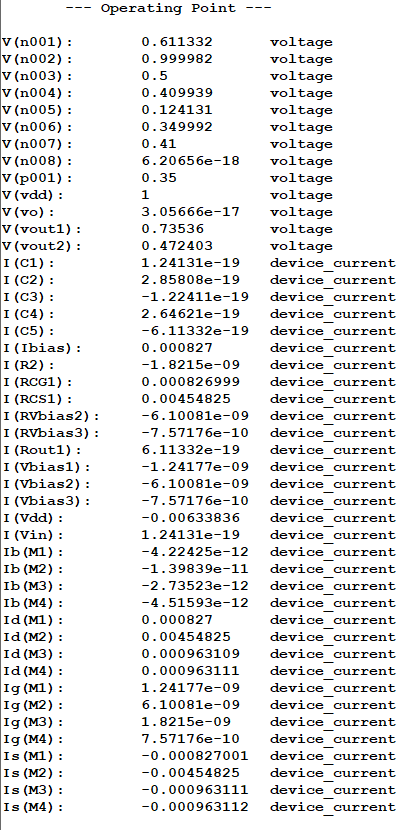
\includegraphics[width=\textwidth]{IMAGENS/ltspice45nm/CMOS45nm_N275_DCop.png}
        \caption{Ponto de operação DC do simulador.}
        \label{fig:op45_N275}
    \end{subfigure}
    \vskip\baselineskip
    \begin{subfigure}[c]{0.48\textwidth}
        \centering
        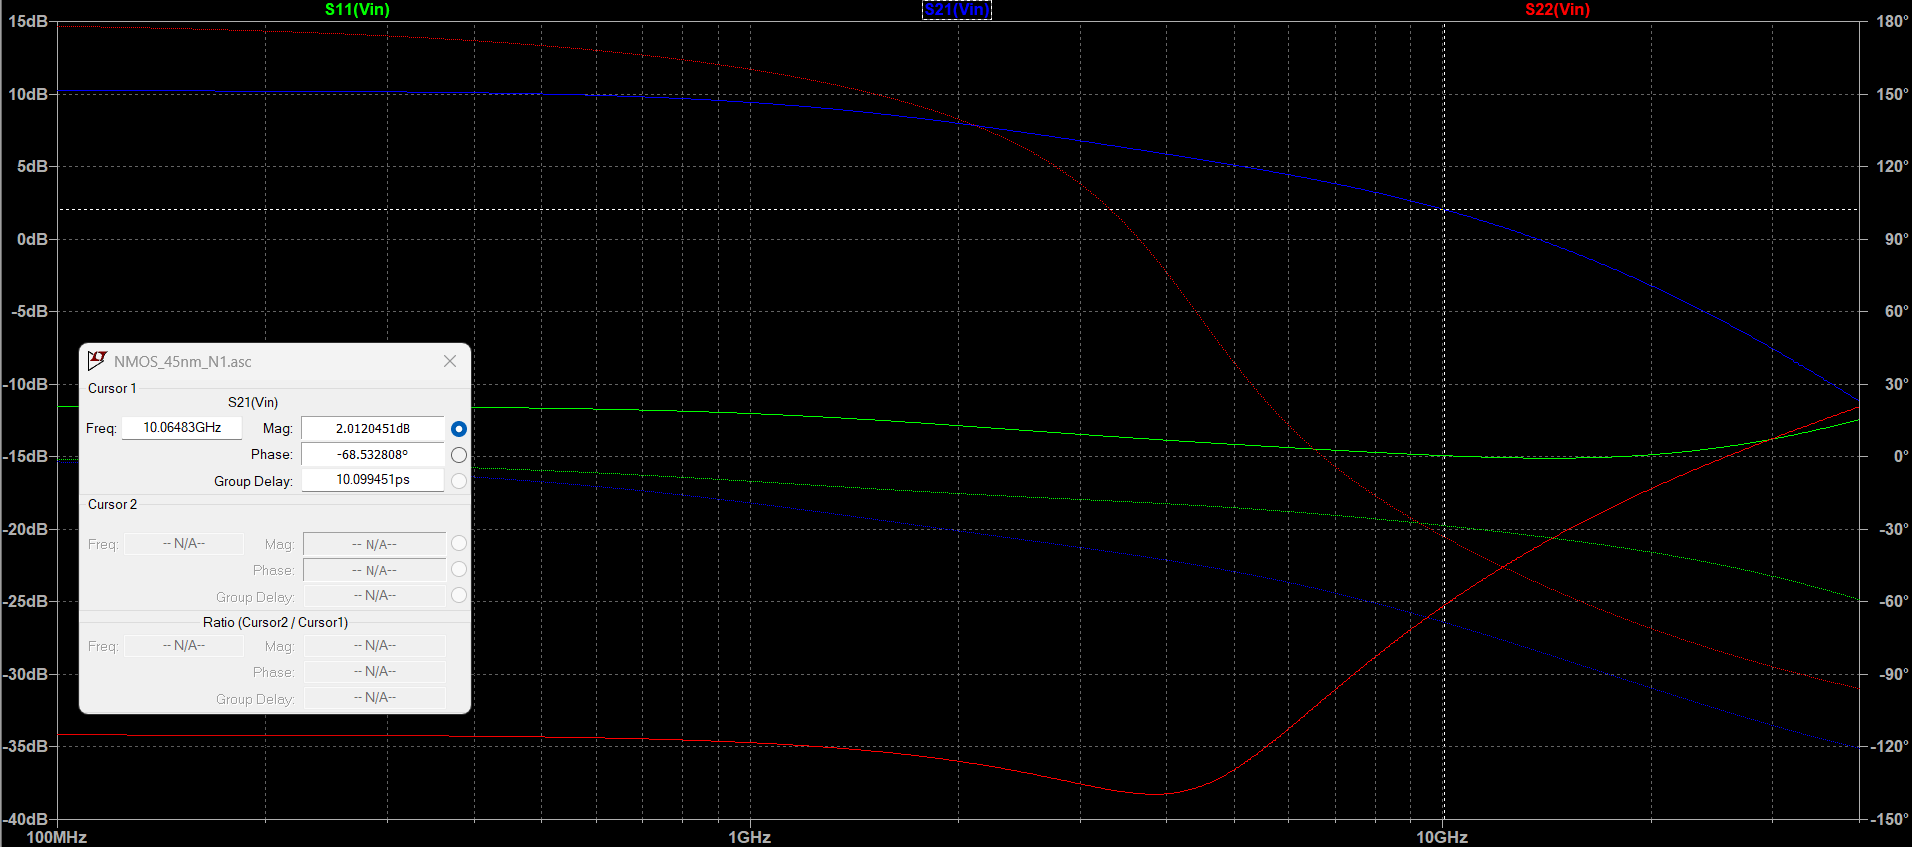
\includegraphics[width=\textwidth]{IMAGENS/ltspice45nm/CMOS45nm_N275_gainSparam.png}
        \caption{Resposta em frequência dos parâmetros S.}
        \label{fig:gain45_N275}
    \end{subfigure}
    \caption{Análise espetral de ruído, ponto de operação DC e coeficientes de transmissão/reflexão para o fator de escala 
    nominal $N=2{,}75$ em tecnologia CMOS de 45\,nm alinhado para a frequência central de 10\,GHz.}
\end{figure}

\subsubsection{Fator de escala \texorpdfstring{$N = 3{,}5$}{N=3.5}}

\begin{figure}[H]
    \centering
    \begin{subfigure}[b]{0.48\textwidth}
        \centering
        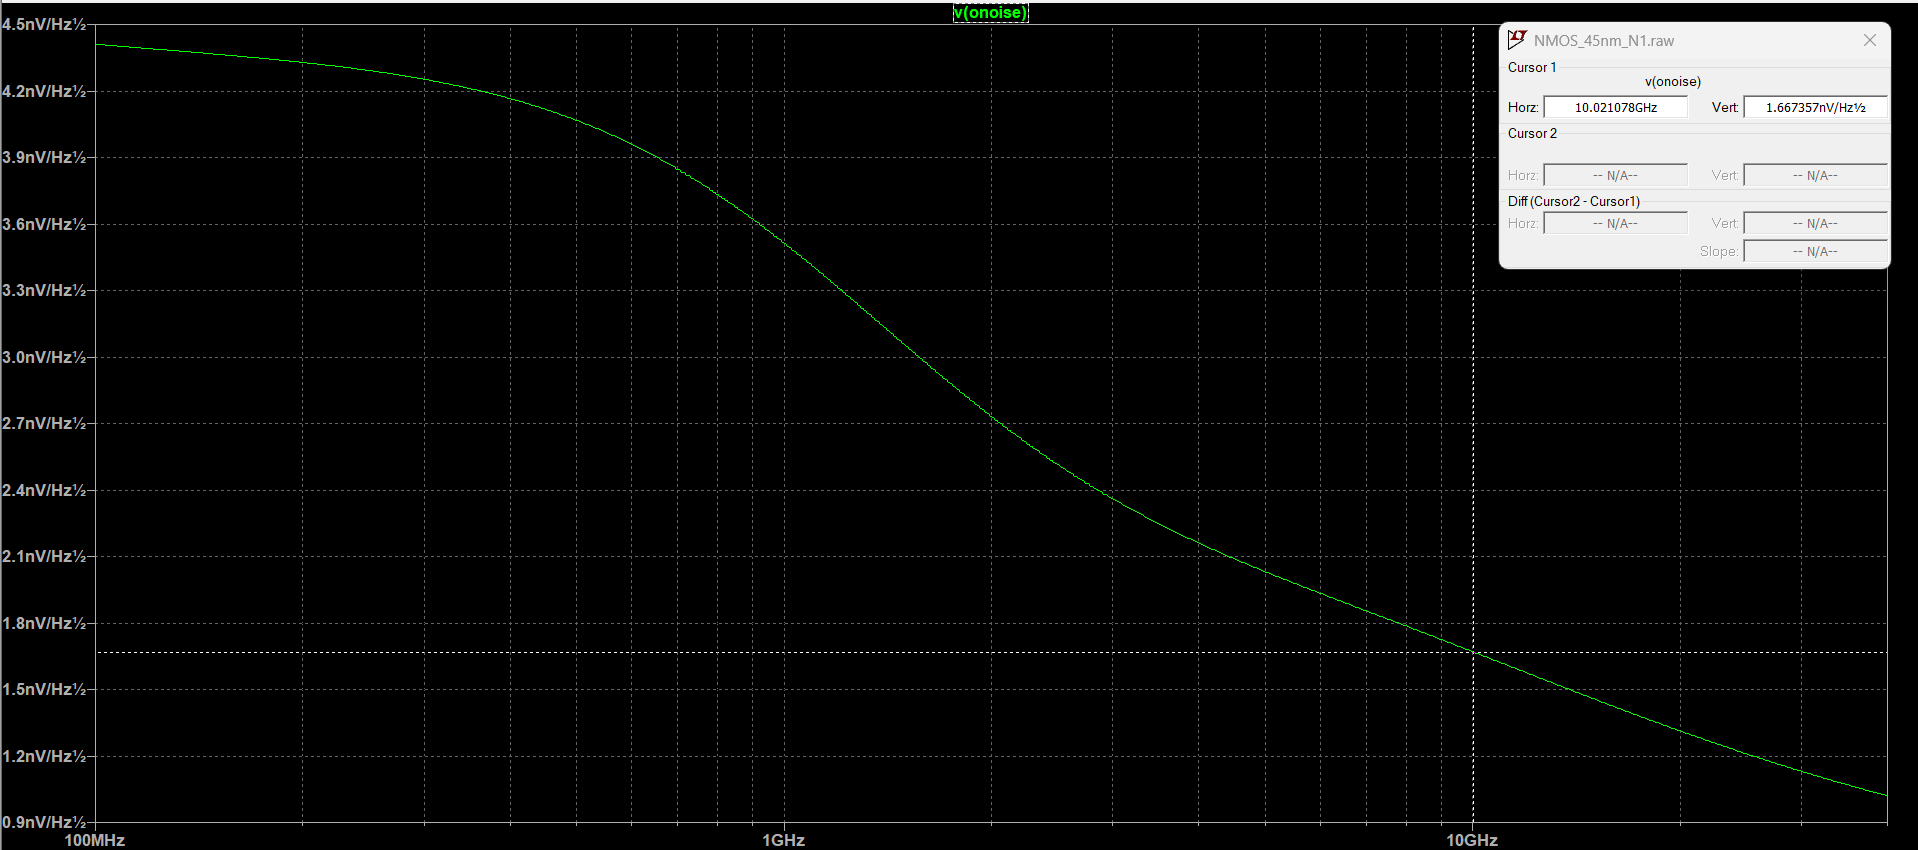
\includegraphics[width=\textwidth]{IMAGENS/ltspice45nm/CMOS45nm_N35_noise.png}
        \caption{Espetro de densidade de ruído.}
        \label{fig:noise45_N35}
    \end{subfigure}
    \hfill
    \begin{subfigure}[b]{0.48\textwidth}
        \centering
        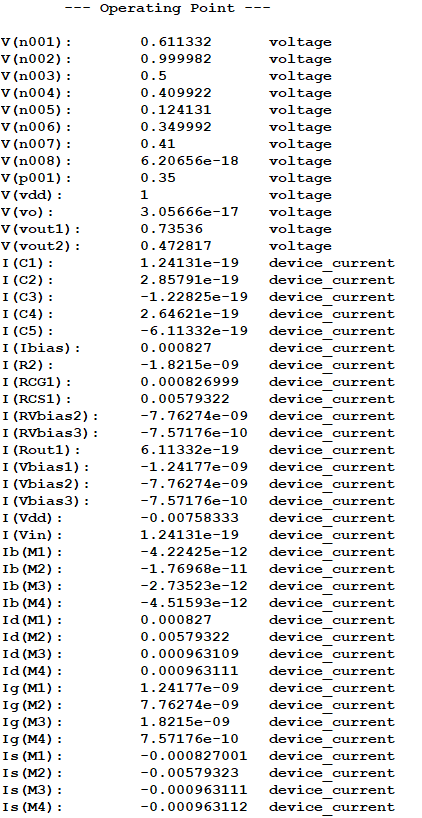
\includegraphics[width=\textwidth]{IMAGENS/ltspice45nm/CMOS45nm_N35_DCop.png}
        \caption{Ponto de operação DC do simulador.}
        \label{fig:op45_N35}
    \end{subfigure}
    \vskip\baselineskip
    \begin{subfigure}[c]{0.48\textwidth}
        \centering
        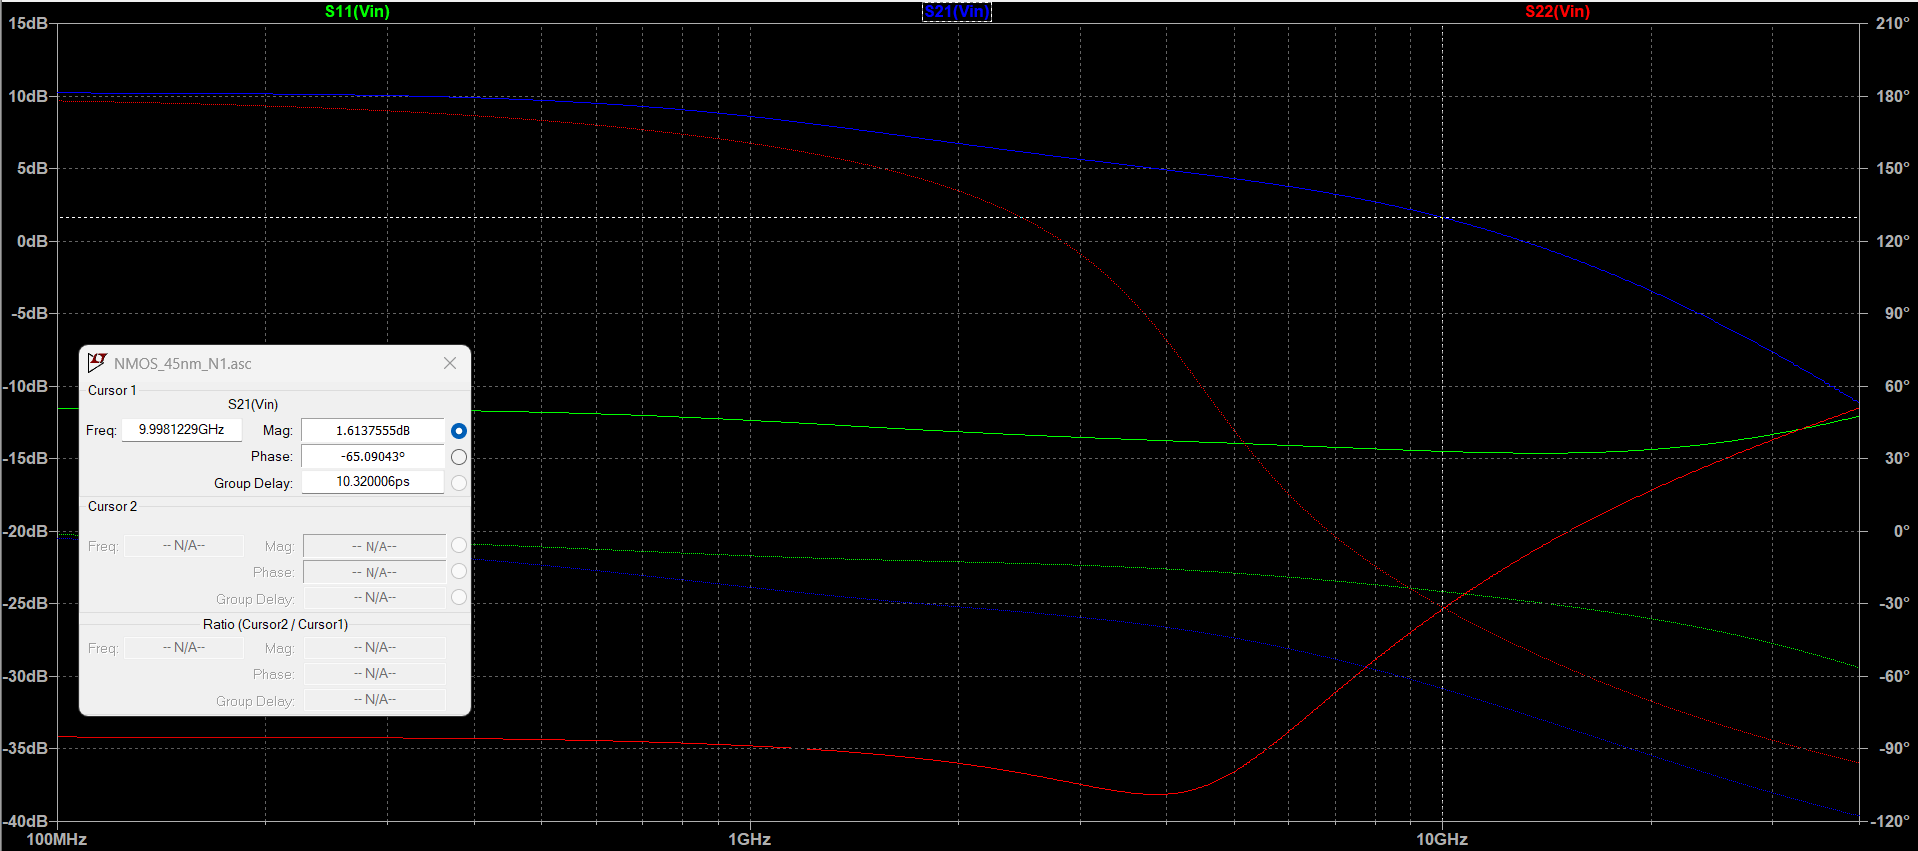
\includegraphics[width=\textwidth]{IMAGENS/ltspice45nm/CMOS45nm_N35_gainSparam.png}
        \caption{Resposta em frequência dos parâmetros S.}
        \label{fig:gain45_N35}
    \end{subfigure}
    \caption{Análise espetral de ruído, ponto de operação DC e coeficientes de transmissão/reflexão para $N=3{,}5$ em tecnologia 
    CMOS de 45\,nm alinhado para a frequência central de 10\,GHz.}
\end{figure}

% ============================================================
\subsection{Comparação dos desempenhos das tecnologias CMOS}
% ============================================================

A Tabela~\ref{tab:comp_tecnologias} sintetiza e cruza os parâmetros de desempenho mais relevantes medidos para as três tecnologias 
CMOS sob o fator de escala de referência fixado em $N = 2{,}75$.

\begin{table}[H]
\centering
\caption{Matriz comparativa de desempenho global entre os nós tecnológicos CMOS para o ponto operativo $N = 2{,}75$.}
\label{tab:comp_tecnologias}
\begin{tabular}{lcccc}
\hline
\textbf{Parâmetro}        & \textbf{350\,nm} & \textbf{65\,nm} & \textbf{45\,nm} & \textbf{Unidade} \\
\hline
$g_m$ (M1)                 & \texttt{???}     & \texttt{???}    & \texttt{???}    & mS \\
$g_{mb}$ (M1)              & \texttt{???}     & \texttt{???}    & \texttt{???}    & mS \\
$Z_{\text{in}}$            & \texttt{???}     & \texttt{???}    & \texttt{???}    & $\Omega$ \\
$g_{ds}$ (M1)              & \texttt{???}     & \texttt{???}    & \texttt{???}    & mS \\
Ganho Intrínseco (M1)      & \texttt{???}     & \texttt{???}    & \texttt{???}    & -- \\
$f_T$ (M1)                 & \texttt{???}     & \texttt{???}    & \texttt{???}    & GHz \\
Ruído Total (V\textsuperscript{2}/Hz) & \texttt{???} & \texttt{???} & \texttt{???} & -- \\
\hline
\end{tabular}
\end{table}

A análise comparativa entre os nós tecnológicos coloca em evidência as tendências fundamentais da física de semicondutores 
amplamente documentadas na literatura analógica. À medida que o comprimento nominal do canal encolhe, a frequência de transição 
$f_T$ experimenta uma subida substancial, reflexo direto da redução drástica das capacidades parasitas intrínsecas dos terminais 
ativos. Esta aceleração é altamente vantajosa para a operação na banda de micro-ondas e RF de alta frequência. 

Contudo, este benefício é severamente contrabalançado pela degradação do ganho intrínseco ($g_m/g_{ds}$), ditado pelo acoplamento 
eletrostático imperfeito do canal, e pelo incremento expressivo da condutância de substrato ($g_{mb}$). Em termos práticos, a 
relevância assumida por $g_{mb}$ nos nós de 65\,nm e 45\,nm redesenha por completo o cálculo de $Z_{\text{in}}$, como formulado 
em~\eqref{eq:zin_65nm}. A consequência direta é que o casamento de entrada deixa de estar indexado em exclusivo à variável $g_m$, 
exigindo o controlo rigoroso do efeito de corpo.

Sob a perspetiva da modelação do ruído, a contração da tensão de alimentação ($V_{DD}$) associada a uma maior densidade de 
corrente eleva o ruído térmico induzido no dreno (*channel thermal noise*). Em simultâneo, o ruído resistivo induzido na porta 
(governado por $r_g$) escala de importância devido à diminuição da espessura física do óxido e da largura dos dedos de polissilício. 
A Figura de Ruído total do LNA balun passa a ser condicionada por imperfeições e acoplamentos internos que eram estatisticamente
irrelevantes na tecnologia madura de canal longo de 350\,nm.

Em suma, a transição para modelos avançados BSIM4 em 45\,nm e 65\,nm dita que o processo clássico de dimensionamento em papel se 
torne um vetor puramente indicativo e inicial. O cumprimento estrito das metas de projeto, especificamente $Z_{\text{in}} = 
50~\Omega$ e imunidade ao ruído, requer necessariamente o recurso a fluxos de simulação iterativos assistidos por computador, 
calibrando as geometrias face às condutâncias parasitas não-lineares reportadas pelo simulador.